% LaTeX mintafájl szakdolgozat és diplomamunkáknak az
% SZTE Informatikai Tanszekcsoportja által megkövetelt
% formai követelményeinek megvalósításához
% Modositva: 2011.04.28 Nemeth L. Zoltan
% A fájl használatához szükséges a magyar.ldf 2005/05/12 v1.5-ös vagy késõbbi verziója
% ez letölthetõ a http://www.math.bme.hu/latex/ weblapról, a magyar nyelvû szedéshez
% Hasznos információk, linekek, LaTeX leirasok a www.latex.lap.hu weboldalon vannak.
%


\documentclass[12pt]{report}

%Magyar nyelvi támogatás (Babel 3.7 vagy késõbbi kell!)
\usepackage[utf8]{inputenc}
\usepackage{t1enc}
\usepackage[magyar]{babel}
% A formai kovetelmenyekben megkövetelt Times betûtípus hasznalata:
\usepackage{times}

%Az AMS csomagjai
\usepackage{amsmath}
\usepackage{amssymb}
\usepackage{amsthm}

%A fejléc láblécek kialakításához:
\usepackage{fancyhdr}

%Természetesen további csomagok is használhatók,
%például ábrák beillesztéséhez a graphix és a psfrag,
%ha nincs rájuk szükség természetesen kihagyhatók.
\usepackage{graphicx}
\usepackage{psfrag}

%tetelszerû környezetek definiálhatók, ezek most fejezetenkent egyutt szamozodnak, pl.
\newtheorem{tet}{tetel}[chapter]
\newtheorem{defi}[tet]{Definíció}
\newtheorem{lemma}[tet]{Lemma}
\newtheorem{áll}[tet]{Állítás}
\newtheorem{köv}[tet]{Következmény}

%Ha a megjegyzések és a példak szövegét nem akarjuk dõlten szedni, akkor
%az alábbi parancs után kell õket definiální:
\theoremstyle{definition}
\newtheorem{megj}[tet]{Megjegyzés}
\newtheorem{pld}[tet]{Példa}

%Margók:
\hoffset -1in
\voffset -1in
\oddsidemargin 35mm
\textwidth 150mm
\topmargin 15mm
\headheight 10mm
\headsep 5mm
\textheight 230mm


% saját package-ek:
 \usepackage{hyperref}
 \usepackage{float}
\usepackage{alltt}
\usepackage{listings}
\usepackage{textcomp}
\usepackage{multirow}
\usepackage{booktabs}
\usepackage{makecell}
\usepackage{tikz}
\usepackage{pgfplots}
\usepackage{indentfirst} % Az első bekezdés is legyen behúzott
\pgfplotsset{compat=1.18}
\setlength{\parindent}{1cm} % Behúzás mértéke (1 cm)
\usepackage{csquotes}






% Referencing
\usepackage[
backend=biber,
style=numeric,
sorting=none
]{biblatex}
\addbibresource{references.bib}


% Listings beállítások
\lstset{
  basicstyle=\ttfamily\small,
  breaklines=true,
  frame=single,
  rulecolor=\normalcolor,
  columns=fullflexible,
  keepspaces=true,
  showstringspaces=false,
  captionpos=b,
  aboveskip=1em,
  belowskip=1em,
  % backgroundcolor=\color{gray!10},
}

\title{
     A nagy nyelvi modellek szemantikus képességeinek konzisztenciájának vizsgálata
}

\begin{document}

%A FEJEZETEK KEZDÕOLDALAINAK FEJ ES LÁBLÉCE:
%a plain oldalstílust kell átdefiniálni, hogy ott ne legyen fejléc:
\fancypagestyle{plain}{%
	%ez mindent töröl:
	\fancyhf{}
	% a láblécbe jobboldalra kerüljön az oldalszám:
	\fancyfoot[R]{\thepage}
	%elválasztó vonal sem kell:
	\renewcommand{\headrulewidth}{0pt}
}

%A TÖBBI OLDAL FEJ ÉS LÁBLÉCE:
\pagestyle{fancy}
\fancyhf{}
\fancyhead[L]{A nagy nyelvi modellek szemantikus képességeinek konzisztenciájának vizsgálata}
\fancyfoot[R]{\thepage}

%A címoldalra se fej- se lábléc nem kell:
\thispagestyle{empty}

\begin{center}
	\vspace*{1cm}
	\begin{Large}
		\bf Szegedi Tudományegyetem
	\end{Large}

	\vspace{0.5cm}

	\begin{Large}
		\bf Informatikai Intézet
	\end{Large}

	\begin{Large}
		\bf Számítógépes Algoritmusok és Mesterséges Intelligencia Tanszék
	\end{Large}

	%\begin{Large}
	%	\bf Nyelvtechnológiai csoport
	%\end{Large}


	\vspace*{3cm}


	{\LARGE\bf \begin{Large}
		\bf
		A nagy nyelvi modellek szemantikus képességeinek konzisztenciájának vizsgálata
		\end{Large}}


	\vspace*{0.5cm}


	{\LARGE\bf \begin{Large}
		\bf
		Reviewing the Consistency of Semantical Capabilities of Large Language Models
		\end{Large}}

	\vspace*{2.4cm}


	{\Large Szakdolgozat}

	%\vspace*{4cm}

	%\newpage

	\thispagestyle{empty}

	% vagy {\Large Diplomamunka}

	\vspace*{2cm}

	%Értelemszerûen megváltoztatandó:
	{\large
		\begin{tabular}{c@{\hspace{2cm}}c}
			\emph{Készítette:}                & \emph{Témavezetõ:}         \\
			\bf{Fábián Bernát}               & \bf{Dr. Berend Gábor Iván} \\
			Programtervező informatikus szakos & egyetemi docens              \\
			hallgató                           &
		\end{tabular}
	}
%\end{center}

%\vspace*{3.6cm}
%\begin{center}
%	\begin{Large}
%		\bf Informatikai Intézet
%	\end{Large}

%	\begin{Large}
%		\bf Számítógépes Algoritmusok és Mesterséges Intelligencia Tanszék
%	\end{Large}

	% \begin{Large}
	% 	\bf Nyelvtechnológiai csoport
	% \end{Large}

%	\vspace*{3.6cm}

	{\Large
		Szeged
		\\
		\vspace{2mm}
		2025
	}
\end{center}
\clearpage



%A \chapter* parancs nem ad a fejezetnek sorszámot
\chapter*{Feladatkiírás}
%A tartalomjegyzékben mégis szerepeltetni kell, mint szakasz(section) szerepeljen:
\addcontentsline{toc}{section}{Feladatkiírás}

A hallgató feladata egy olyan keretrendszer megvalósítása, amely lehetővé teszi a nagy nyelvi modellek szemantikával kapcsolatos képességeinek konzisztenciájának vizsgálatát. A kiértékelés során azt vizsgálja a keretrendszer, hogy a nagy nyelvi modellek válaszai milyen érzékenységet mutatnak olyan invarianciákra, amelyek az emberi válaszadásra nincsenek befolyással. A kísérletek során a nagy nyelvi modellek azzal kapcsolatos érzékenységének vizsgálata a cél, hogy mennyiben érzékenyek a nagy nyelvi modellek a Word-in-Context nevű feladat megoldása során az egyes inputokban szereplő mondatpárosok sorrendjének megcserélésére.

A hallgató megoldási terve:
A Word-in-Context probléma megismerése, a jelenlegi legjobb megoldások áttekintése és összehasonlítása, valamint annak a megvizsgálása, hogy generatív nyelvi modellek mennyire teljesítenek jól a Word-in-Context benchmarkon determinisztikus és izolált válaszadás esetén, kóddal automatizálva a promptolást és a válaszfeldolgozást. Valamint egy WiC kiértékelő Python modul megtervezése, implementálása és tesztelése.
\begin{itemize}
	\item Ismerje meg az NLP és a nagy nyelvi modellek fogalomrendszerét.
	\item Általa választott modelleken vizsgálja meg, hogy mennyire adnak a Gold Standarddal megegyező választ, és hogy mennyire érzékenyek arra, hogy
	      \begin{verbatim}Does the word `w` mean the same thing
        in sentences `s1` and `s2`?\end{verbatim}
	      formájú kérdésekben a két mondatot fordítva kapják meg, ahol $w$ egy szó, $s1$ az első példamondat, és $s2$ a második példamondat. Tehát a modellnek az "Ugyanazt jelenti-e a szó az $A$ és $B$ mondatban?" kérdésre a válasza ugyanaz-e, mint a "Ugyanazt jelenti-e a szó a $B$ és $A$ mondatban?" kérdésre.
	\item Tervezze meg, implementálja és tesztelje a kontextusalapú szójelentés-felismerő rendszerét a \href{https://pilehvar.github.io/wic/}{WiC adathalmaz} alapján. Az adatok letöltése után végezze el a szükséges adattranszformációkat, az adattisztítási feladatokat, szűrje ki a felesleges vagy használhatatlan adatok körét, illetve készítse el az elemzéshez a kész adatállományt.
	\item Az elért eredményeiről készítsen statisztikai összesítéseket.
\end{itemize}
Elvégzett munkáit a Szakdolgozat keretében dokumentálja.

\clearpage

\chapter*{Tartalmi összefoglaló}
\addcontentsline{toc}{section}{Tartalmi összefoglaló}

\begin{itemize}
\item \textbf{A téma megnevezése}

    Egyrészt a kontextusalapú szójelentés-felismerés (Word-in-Context, WiC) feladat, tágabb értelemben a szójelentés-egyértelműsítés (Word Sense Disambiguation,
    WSD), nyelvtechnológiai (NLP) módszereket és eszközöket használva. Másrészt a generatív nyelvi modellek, a promptolásának, a válaszgenerálásnak és a válaszok feldolgozásának automatizálása.

\item \textbf{A megadott feladat megfogalmazása}

      A feladat megvizsgálni, hogy a Mohammad Taher Pilehvar által összeállított és publikált \href{https://pilehvar.github.io/wic/}{Word-in-Context feladatot} önállóan választott ingyenes és nyílt forráskódú generatív nyelvi modellek mennyire jól oldják meg. A modellek válaszainak összehasonlítása és elemzése, ehhez egy saját adatfeldolgozó és  kiértékelő rendszer megtervezése, implementálása Python nyelven, majd tesztelése. A rendszernek képesnek kell lennie a pontosság mellett a fedés és a precizitás értékét megadni, továbbá tévesztési mátrixot készíteni a predikciók eloszlásáról, az alábbi négy osztályba sorolva:
      \begin{itemize}
        \item \textbf{TP (True Positive):} Azok az esetek, amikor a modell helyesen ismeri fel, hogy a szó jelentése megegyezik a két mondatban.
        \item \textbf{FP (False Positive):} Azok az esetek, amikor a modell tévesen gondolja azt, hogy a szó jelentése megegyezik, pedig valójában eltér.
        \item \textbf{FN (False Negative):} Azok az esetek, amikor a modell nem ismeri fel a jelentésazonosságot, pedig a szó jelentése valójában megegyezik.
        \item \textbf{TN (True Negative):} Azok az esetek, amikor a modell helyesen ismeri fel, hogy a szó jelentése különböző a két mondatban.
      \end{itemize}

\item \textbf{A megoldási mód}
    A megoldásom során törekedtem arra, hogy az bárki által reprodukálható legyen, ezért ingyenesen elérhető és nyílt forráskódú eszközöket (Python, GitHub, Hugging Face) használtam.
      \begin{itemize}
        \item
              A szakdolgozatom első felében kielemeztem az eddigi legjobb modelleket és a legjobb módszereket szójelentés-értelmezés szempontjából és nyílt forráskódú nyelvi modelleket kerestem a LMArena és Hugging Face felületein, továbbá az utóbbiak futtatásának dokumentációját tanulmányoztam.
            \item Összehasonlító teljesítményvizsgálatot végeztem a
            % TODO update-elni Gemma3-ra és QWEN3-ra mindenhol
            \href{https://huggingface.co/microsoft/Phi-4-mini-instruct}{Phi-4-mini-instruct}, \href{https://huggingface.co/google/gemma-2-2b-it}{Gemma-2-2b-it} és a \href{https://huggingface.co/Qwen/Qwen1.5-1.8B-Chat}{Qwen1.5-1.8B-Chat} között egy Google Colab szkriptben.
        \item
              Saját adatfeldolgozó kiértékelő Python modult készítettem a promptolás automatizálásához és a modell válaszok feldolgozására.
        \item A választott modelleket inferenciára bírtam az automatizáló szkriptekkel különböző módokban a szósorrend-érzékenységének és egyéb metrikák összehasonlítására

      \end{itemize}
\item \textbf{Az alkalmazott eszközök}
      \begin{itemize}

        \item Google Colab és PyCharm, Python futtatókörnyezet
        \item Git, GitHub
        \item Hugging Face
        \item Torch és Transformers Python könyvtárak
        \item NLTK és WordNet
        \item CUDA, Accelerate, BERT
        \item Google Táblázatok, Apps Script

      \end{itemize}
      \item \textbf{Módszer}
      \begin{itemize}

        \item Objektum Orientált Python programozás
        \item Clean Code alapelvek Martin és Robert Clean Code c. könyve \cite{martin2008cleancode} alapján

      \end{itemize}
\item \textbf{Az elért eredmények}
        \\
        \begin{itemize}
            \item A szoftver képes a WiC adathalmaz sorainak egyszerű promptokká, kérdésekké alakítására, majd a modellek válaszainak feldolgozására.
        A mintafeladathoz készült feldolgozó modul elvégzi a szükséges adattranszformációkat, az adattisztítási feladatokat és az adat könnyen értelmezhető formába alakítását.

     \item Sikerült átfogó elemzést készítenem 3 Hugging Face-ről
      letölthető generatív nyelvi modell teljesítményéről.
      % Kiértékelő rendszer és függvénykönyvtár, amelynek célja a WiC (Word in Context) adathalmaz feldolgozása és a  feladatok megoldásának vizsgálata különböző nyelvi modellek segítségével. Az alkalmazás arra is képes, hogy elemezze, mennyire érzékenyek ezek a modellek arra, ha a két példamondat sorrendjét felcseréljük.
        \end{itemize}


      Harmadik büszkeségem, hogy algoritmikus módszerekkel 60+ \%-os eredményeket értem el, amely felülmúlja a legtöbb 0-3 milliárd paraméteres általános célú nyelvi modell teljesítményét.

\item \textbf{Kulcsszavak}
        \\
       Word-in-Context, szóbeágyazások, nyelvtechnológia, nyelvi modell, szójelentés-ábrázolás
\end{itemize}

%A tartalomjegyzék:
\tableofcontents

\clearpage

{\Large\bf Motiváció }

\addcontentsline{toc}{section}{Motiváció}
Az informatika és a nyelvtechnológia fejlődésével a generatív mesterséges intelligencia mindennapjaink részévé vált. A mesterséges intelligenciát használó nagy nyelvi modellek kiértékelésére számos benchmark (\textit{teljesítményteszt} vagy \textit{metrika}) fejlődött ki az évek során. A legnépszerűbb ilyen benchmark a
SuperGLUE, amely nyolc, komoly kihívást jelentő feladat elé állítja a nagy nyelvi modelleket. Ebben a papírban a WiC feladatot mutatom be.

A WiC (Word-in-Context) probléma a SuperGlue 8 feladatának egyike. Az emberi szöveget értő nyelvi modellek fejlesztése kiemelten fontos mind az akadémiai kutatásban, mind a gyakorlati alkalmazásokban. Az angol nyelvű szövegek feldolgozása nem csak az angolszász területeken releváns, hanem Magyarországon is, hiszen az angol nyelv használata a számítógépek világában mindennapjaink része. Az egyetem és a helyi vállalatok is aktívan foglalkoznak természetesnyelv-feldolgozási (NLP) megoldásokkal. A munkahelyeken – különösen IT területen – egy jól működő WiC modell jelentős előnyt biztosíthat kódok, dokumentumok, ügyfélkommunikáció vagy akár jogi szövegek értelmezésében, ami kulcsfontosságú lehet például a tudásközpontokban és startup cégeknél is. Egy hatékony WiC modell tehát nemcsak tudományos értékkel bír, hanem gyakorlati alkalmazásokban is közvetlen hasznot hozhat, főleg a nyelvészeti informatikai területen dolgozók számára.
\clearpage

\chapter*{Bevezetés}
\addcontentsline{toc}{section}{Bevezetés}

\section*{Irodalmi áttekintés}

% \begin{itemize}
% 	\item TF-IDF és hasonlósági mérőszámok (baseline módszerek).
% 	\item WordNet, Lesk algoritmus és egyéb WSD technikák: Rövid magyarázat a működésről.
% 	\item Modern neurális módszerek: Transformer alapú modellek (pl. BERT).
% 	\item Ingyenes modellek használata Hugging Face és Ollama segítségével
% 	\item Benchmark adathalmazok és értékelési metrikák: pontosság (accuracy), fedés (recall), precizitás (precision), F1 pontszám (F1-score), tévesztési mátrix (confusion matrix).
% \end{itemize}



A szóbeágyazások tervezésükből adódóan képtelenek modellezni a szavak szemantikájának dinamikus természetét, vagyis azt a tulajdonságot, hogy a szavak potenciálisan különböző jelentéseknek felelhetnek meg. E korlátozás kezelésére számos specializált jelentésreprezentációs technika jelent már meg, mint például a jelentés- vagy kontextualizált beágyazások. Azonban a téma kutatásának népszerűsége ellenére igen kevés olyan értékelési viszonyítási alap létezik, amely kifejezetten a szavak dinamikus szemantikájára összpontosít. A meglévő modellek túllépték az erre a célra szolgáló standard értékelési adatkészlet, a Stanford Kontextuális Szóhasonlóság teljesítménykorlátját. A megfelelő viszonyítási alap hiányának kezelésére készült a nagyszabású, szakértők által összeállított annotációkon alapuló Word in Context adatkészlet, a WiC, amely a szavak kontextustől függő jelentését vizsgálja. A WiC nyilvánosan elérhető a \href{https://pilehvar.github.io/wic/}{WiC: The Word-in-Context Dataset} weboldalon.\cite{pilehvar2019wic}


\section*{A szakdolgozat célja}

A szakdolgozatom elsődleges célja, hogy megvizsgáljam egy pár gondosan megválasztott modellen, hogy mennyire teljesítenek jól a WiC feladaton, és mennyire érzékenyek arra, ha a mondatokat felcserélve kapják meg. Tehát mennyire befolyásolja a döntésüket a szavak sorrendje. Mindezt úgy, hogy az egyetlen kóddal futtatható és jól dokumentálható legyen, és a kérdéseket egyesével kell beadni, hogy az előző válaszok ne befolyásolják a modell döntését, csak a saját tudására, tehát az előtanítása alatt szerzett információra támaszkodjon. Tehát futás közben nem történik tanítás.


\chapter{A WiC probléma}
\phantomsection
\addcontentsline{toc}{section}{A WiC adathalmaz}

\section{A többértelműség problémája a természetes nyelvekben}

A természetes nyelvekben a programozási nyelvekkel ellentétben egy szónak több, egymástól teljesen elkülönülő jelentése is lehet. Például az "egér" szó jelenthet egy számítógépes perifériát vagy egy állatot, és a helyes értelmezéshez a környező szavakat ismerni kell. Az ilyen jellegű többértelműségek automatikus feloldása az egyik központi problémája a természetes nyelvi rendszerek fejlesztésének.


\section{A WiC probléma}
Az emberi nyelvekben a többértelmű szavak attól függően, hogy milyen szövegkörnyezetben fordulnak elő, több, esetenként egymással össze nem függő jelentést is hordozhatnak. Míg korábban a statikus szóbeágyazások, mint például a Word2vec és a GloVe voltak elterjedtek a szójelentés feloldására, ma már elavult módszereknek számítanak. Ezek a statikus szóbeágyazások tervezésükből adódóan nem képesek modellezni a szavak szemantikájának dinamikus természetét, vagyis azt a tulajdonságot, hogy a szavak potenciálisan különböző jelentéseknek felelhetnek meg. Egy szóhoz mindig ugyanazt a szóvektort rendelik, kontextustól függetlenül. A kontextualizált szóbeágyazások kísérletet tesznek ennek a korlátnak a feloldására azáltal, hogy dinamikus reprezentációkat számítanak ki a szavakhoz, amelyek a szövegkörnyezet alapján képesek alkalmazkodni. Ilyen szóbeágyazás transzformer például a BERT, ám ennek is megvannak a korlátai. A mai igazán modern megoldások viszont már mély tanulást és jellemzően neurális hálókat használnak a modellek szójelentés-értelmező képességeinek fejlesztésére.

A WiC feladat lényege, hogy egy adott szó két különböző mondatbeli előfordulásáról eldöntse, hogy azonos értelemben szerepel-e. A természetes nyelvi feldolgozásban.
\footnote[1]{Természetesnyelv-feldolgozás, számítógépes nyelvészet és nyelvtechnológia néven is hivatkoznak rá, angolul NLP}


\section{Egy rendszer feladata a WiC adathalmazon}
Amikor valaki kiértékelő rendszert fejleszt a WiC benchmarkra, annak feladata a szavak szándékozott jelentésének azonosítása. A WiC egy bináris osztályozási feladatként van megfogalmazva. Adott egy többjelentésű szó, amely mindkét mondatban előfordul, továbbá egy szófaj címke, kettő index és két szövegrészlet. Egy rendszer feladata, hogy meghatározza, hogy a szó ugyanabban a jelentésben használatos-e mindkét mondatban. A $w$ célszó minden esetben csak egy ige vagy főnév lehet. A célszóhoz két eltérő szövegkörnyezet tartozik. Ezen szövegkörnyezetek mindegyike a $w$ egy specifikus jelentését váltja ki. A feladat annak megállapítása, hogy a $w$ előfordulásai a két szövegkörnyezetben ugyanannak a jelentésnek felelnek-e meg, vagy sem. Tehát a célszó ugyanazt a jelentést hordozza-e két különböző szövegkörnyezetben, vagy eltérőt. Ez egy összetett NLP probléma, mivel ötvözi a szójelentés-egyértelműsítés (Word Sense Disambiguation, WSD) és a kontextuális beágyazások elemeit, így a szójelentés-egyértelműsítés végrehajtásaként is értelmezhető.

\section{Bináris osztályozás}
A WiC feladat egy bináris osztályozási (binary classification) problémaként van megfogalmazva: el kell dönteni, hogy egy adott szó két különböző mondatbeli előfordulása ugyanabban az értelemben szerepel-e.
A bináris osztályozási feladatok problémakörében is változnak a trendek olyan szempontból, hogy egyre inkább a neurális hálók és nagy nyelvi modellek az elterjedtek bináris osztályozási feladatokra is. A Lesk-algoritmus~\cite{lesk1986automatic} egy klasszikus szóértelem-felismerő módszer, amely a szótári definíciók és a kontextus összevetésével próbálja meghatározni a szó legmegfelelőbb jelentését. A legjobbak mégis az olyan, kifejezetten emberi szöveg megértésére specializálódott nagy nyelvi modellek, mint például a GPT-4.5 és a Gemini-2.5 - 2025 telén.

\label{wic:dataset}
\section{A WiC adathalmaz eredete}

A \href{https://pilehvar.github.io/wic/}{Word in Context adathalmaz} egy jó minőségű, nyelvészeti szakértők által készített benchmark adathalmaz. A mondatok a WordNetből, a VerbNetből és a Wikiszótárból származnak.
A WiC adathalmaz segítségével megvizsgálhatjuk, hogy egy rendszer (modell, algoritmus) mennyire képes a szavak jelentését megérteni különböző kontextusokban. A WiC feladat része a SuperGlue~\cite{sarlin2020superglue} Benchmarknak, amely egy széles körben elfogadott benchmark nyelvi modellek kiértékelésére. 8 feladatból áll:
\begin{itemize}
	\item  BoolQ (Boolean Questions)
	\item  CB (CommitmentBank)
	\item COPA(Choice of Plausible Alternatives)
	\item MultiRC (Multi-Sentence Reading Comprehension)
	\item ReCoRD(Reading Comprehension with Commonsense Reasoning Dataset)
	\item RTE(Recognizing Textual Entailment)
	\item \textbf{WiC(Word-in-Context)}
	\item  WSC (Winograd Schema Challenge)
\end{itemize}

A SuperGLUE a GLUE továbbfejlesztett változata, amelyet 2019-ben vezettek be, mivel a GLUE feladatait a legmodernebb modellek (pl. BERT) már túl jól megoldották. ~\cite{wang2020superglue}
Ez az egyik legszélesebb körben elfogadott benchmark, amelyen számos nyelvi modell teljesítményét vizsgálták.
A WiC halmaz fel van osztva tanító, validációs és teszthalmazra, ezért gépi tanításra egyszerűen felhasználható. Ezt segíti elő az is, hogy az összes mondat tokenekre bontott, tabulált és egységesek az írásjelek is.
A modelleket hasonlóan tanítják, mint ahogy az iskolában tanulnak a diákok.
A benchmarkok feladatait jellemzően 3 részre vágják:
tanító, validációs és teszthalmazra. Ennek az aránya eltérő lehet, de a tanítónak jóval nagyobbnak kell lennie, mint a másik kettőnek, és a teszthalmaznak nagyobbnak kell lennie, mint a validációs halmaznak. 80-10-10\%-os eloszlás a standard, ezzel, vagy hasonló eredménnyel érhetőek általában el a legjobb eredmények.

A tanító adatbázist a korábbi iskolai példára visszatérve úgy képzelhetjük el, hogy ez a leadott anyag. A validációs halmaz olyan, mint egy mintavizsga, minta ZH. A teszthalmaz pedig a végső megmérettetés, a vizsga. Fontos, hogy a teszthalmazon sose tanítsuk a modelleket, és sose legyen átfedés a halmazok között. Ez ugyanis magoláshoz vezet, és a modell nem lesz képes általánosítani.

\begin{table}[H]
    \centering
    \caption{A WiC adathalmaz tesztkészletének néhány bejegyzése}
    \label{tbl:wic_peldak} % Egyedi címke a táblázathoz
    \begin{tabular}{llcp{0.33\textwidth}p{0.33\textwidth}} % Oszlopdefiníciók: l=balra, c=középre, p{szélesség}=paragrafus adott szélességgel
        \hline
        \textbf{Szó} & \textbf{Szófaj} & \textbf{Index} & \textbf{1. Példamondat} & \textbf{2. Példamondat} \\
        \hline
        defeat      & N      & 4-4       & It was a narrow defeat.                             & The army's only defeat.                                             \\
        groom       & V      & 0-1       & Groom the dogs.                                     & Sheila groomed the horse.                                            \\
        penetration & N      & 1-1       & The penetration of upper management by women.       & Any penetration, however slight, is sufficient to complete the offense. \\
        hit         & V      & 1-3       & We hit Detroit at one in the morning but kept driving through the night. & An interesting idea hit her.                                         \\
        \hline
    \end{tabular}
\end{table}

\subsection{Eddigi legjobb modell-teljesítmények a WiC adathalmazon}
A WiC adathalmazon számos modellt teszteltek, amelyek túlnyomórészt 60\% feletti eredménnyel kategorizálták helyesen a mondatokat.
A legjobb eredményt a SenseBERT-large rendszerrel érték el, külső erőforrások használatával. Ez az eredmény megközelíti a kézi, emberi szintű kiértékelést, melynek a felső határa 80\% körüli. A kézi kiértékelésnek és a SenseBERT megoldásának egyszerűsített változatát én is elvégeztem.


% Requires: \usepackage{booktabs}
\begin{table}[h]
    \centering
    \begin{tabular}{l l c}
        \toprule
        \textbf{Kategória} & \textbf{Implementáció} & \textbf{Pontosság \%} \\
        \midrule
        \multicolumn{3}{l}{\textbf{Sentence-level contextualised embeddings}} \\
        SenseBERT-large\textsuperscript{†} & Levine et al (2019) & 72.1 \\
        KnowBERT-W+W\textsuperscript{†} & Peters et al (2019) & 70.9 \\
        RoBERTa & Liu et al (2019) & 69.9 \\
        BERT-large & Wang et al (2019) & 69.7 \\
        Ensemble & Gari Soler et al (2019) & 66.7 \\
        ELMo-weighted & Ansell et al (2019) & 61.2 \\
        \midrule
        \multicolumn{3}{l}{\textbf{Word-level contextualised embeddings}} \\
        WSDT\textsuperscript{†} & Loureiro and Jorge (2019) & 67.7 \\
        BERT-large & WiC's paper & 65.5 \\
        Context2vec & WiC's paper & 59.3 \\
        Elmo & WiC's paper & 57.7 \\
        \midrule
        \multicolumn{3}{l}{\textbf{Sense representations}} \\
        LessLex & Colla et al (2020) & 59.2 \\
        DeConf & WiC's paper & 58.7 \\
        S2W2 & WiC's paper & 58.1 \\
        JBT & WiC's paper & 53.6 \\
        \midrule
        \multicolumn{3}{l}{\textbf{Sentence level baselines}} \\
        Sentence Bag-of-words & WiC's paper & 58.7 \\
        Sentence LSTM & WiC's paper & 53.1 \\
        \midrule
        \multicolumn{3}{l}{\textbf{Random baseline (véletlenszerű kiértékelés)}} \\
        & 50.0 \\
        % TODO: kiegészíteni a saját eredményemmel
        % \midrule
        % \multicolumn{3}{l}{\textbf{Fábián Bernát kézi kiértékelés}} \\
        % & xx.x
        % \multicolumn{3}{l}{\textbf{Saját PyCharmos implementáció kiértékelés}} \\
        % & 60.x
        \bottomrule
    \end{tabular}
    	\caption{Forrás: \href{https://pilehvar.github.io/wic/}{The Word-in-Context Dataset}}

    \label{tab:state_of_the_art}
\end{table}


\clearpage


\section{Nagy nyelvi modellek}

A nagy nyelvi modell (angolul Large Language Model, LLM) olyan számítási modell, amely képes értelmes szöveg generálására vagy más természetes nyelvi feldolgozási feladatok elvégzésére. Ezek a modellek egy rendkívül költséges folyamat révén, hatalmas mennyiségű szöveges adat feldolgozásával és mélytanulási technikák alkalmazásával sajátítják el a nyelv megértését és előállítását. Az LLM-ek, mint például az OpenAI GPT-sorozata, a Google Gemini vagy a Meta LLaMA modelljei, különböző architektúrákat használnak, de leggyakrabban a transzformer alapú megközelítést alkalmazzák. Mint nyelvi modellek, az LLM-ek úgy sajátítják el ezeket a képességeket, hogy óriási mennyiségű szövegből, egy önfelügyelt és egy félig felügyelt tanulási folyamat során, statisztikai összefüggéseket tanulnak meg. Ezek a modellek  képesek összetett feladatok elvégzésére, mint például szövegfordítás, összefoglalás, információ-kinyerés, kérdés-válasz és kreatív szövegalkotás. Finomhangolás által specializált feladatokra. Nagy nyelvi modelleknek jellemzően az 50 milliárd paraméteresnél nagyobb modelleket hívják. Az ennél kisebb modelleket inkább csak nyelvi modelleknek hívom.

Inputként kap egy promptot, egy legfeljebb \texttt{n} token hosszúságú szöveget, ahol az \texttt{n} függ a modelltől és a paraméterezéstől. Erre fog legfeljebb \texttt{m} hosszúságú válaszban inferenciával, azaz következtetéssel válaszolni. Azért hívják modellnek a modelleket, mert az emberi nyelvet és kommunikációt utánozzák (modellezik).

Forrás: \href{https://hu.wikipedia.org/wiki/Nagy_nyelvi_modell}{Wikipédia}

\subsection{Chatbot Arena, vagy LMSYS - nagy nyelvi modelleket összehasonlító platform}
Kutatómunkám első lépéseként utánanéztem, hogy melyik modellek a legjobbak angol nyelvű instruction following feladatokban. Ehhez a \href{https://lmarena.ai/}{LMArenát}~\cite{chiang2024chatbot} megfelelő referenciának tartottam, mert ez az oldal igen lenyűgöző módon minden ismertebb ingyenes nagy nyelvi modellhez API-n keresztüli limitált hozzáférést biztosít: 2025. május 16-án 101 modell API-ja volt kipróbálható az oldalon keresztül több tucatnyi cégtől, a ranglétrán pedig 241 modell teljesítményét mérhetjük össze különböző kategóriák alapján emberi szavazatok alapján, amely több mint 1.5 millió ember szavazatán alapszik.
A folyamatosan frissülő rangsor menüben az opciók közül az "Instruction Following" és az "English" kategóriát vizsgáltam meg, mert a problémám ehhez a területhez áll a legközelebb.


Az oldalon található modellek mind elérhetőek és kipróbálhatóak, és általában saját, felhasználóbarát webes felületük is van, amely személyre szabható, elmenthetőek a korábbi beszélgetéseink, és egyéb kényelmes szolgáltatásokkal kecsegtetnek. Azonban fontos észben tartanunk, hogy ezeket a felületeket fejlesztő cégek bármilyen publikus webes forrást felhasználhatnak a modelljeik tanításához, beleértve a chatben megadott információt.
A nagy cégeknek, mint például a Google-nek, az OpenAI-nak és a DeepSeek-nek is vannak nyílt forráskódú, jó minőségű modelljeik, melyek hatalmas adathalmazokon be vannak tanítva. Például a GPT-3 tanítása során a Common Crawl Wikipédiát, WebText2 reddit posztokból és linkjeiből kinyert adatokat, internetes könyveket és az angol nyelvű wikipédiát is felhasználták.~\cite{springboard2023gpt3} Régebben a New York Times termékeit is nagy mennyiségben használták, ám a hírlapíró cég ezt felhasználási feltételeiben megtiltotta.~\cite{verge2023nytai}

A nagy tech cégek, mint a Meta és az X, felhasználják a közösségi médiára feltöltött adatainkat a modelljeik fejlesztéséhez. A Google pedig a felhasználási feltételeit is többször megváltoztatta, hogy felhasználhassa szolgáltatásainak felhasználói adatait az AI termékei fejlesztéséhez. ~\cite{tan2024terms}


A Hugging Face~\cite{wolf2019huggingface} [\href{https://huggingface.co/models}{több mint 1.7 millió modellt}] és [\href{https://huggingface.co/datasets}{csaknem 400 ezer adathalmazt}] kínál különféle gépi tanulási feladatokra, beleértve a természetes nyelvfeldolgozást, képfeldolgozást és kódgenerálást is. Ezek a modellek nyilvánosan elérhetők és szabadon használhatók.
Előnyük, hogy nyílt forráskódúak, így tetszőlegesen módosíthatóak - habár alapos szakértelem kell hozzájuk. Emellett biztonságosak: letölthetőek saját gépre, kódból futtathatóak anélkül, hogy egy szerverrel kommunikálnának. Emiatt privát adatot is be lehet nekik adni. Jellemzően minél kisebb a paraméterszámuk, annál gyengébb a visszaemlékező képességük, rövidebb válaszokat részesítenek előnyben, és annál gyakrabban követnek el hibákat vagy nyelvi torzulásokat - például nyelvtani hibákat, kódban szintaktikai hibákat, inkoherens (összefüggéstelen, logikailag következetlen) válaszokat. A kvantálás általában csak a népszerűbb/nagyobb modelleknél (pl. Llama, Gemma, Mistral) elérhető, és gyakran közösségi kontribúciók eredménye (nem hivatalos verziók). A kvantálás a modell súlyait alacsonyabb bitmélységűre (pl. 32 → 8/4 bit) konvertálja, ami csökkenti a memóriaigényt és gyorsítja a következtetést. Emiatt könnyen félrevezethetőek és könnyen hallucinálnak is. Összefoglalva hátrányaik a
\begin{itemize}
	\item
	      korlátozott kontextusmegértés a csökkentett bitmélység miatt, ezért nehezebben követik a hosszú gondolatmeneteket,
	\item
	      gyenge memóriájuk, elfelejtik a korábbi információkat,
	\item
	      és túlzott általánosítás is jellemző rájuk.
\end{itemize}

\clearpage

\section*{Fogalmak}

\addcontentsline{toc}{section}{Nyelvi modell alapfogalmak}

Ahhoz, hogy nagy nyelvi modelleket ki tudjunk értékelni, meg kell ismernünk néhány alapfogalmat.

\subsection{A prompt}
A prompt alatt az informatikában egy nagy nyelvi modell számára beadott olyan inputot értünk, amelyre a modell egy előre meghatározott kimenetet generál. Működési elve lényegében ugyanaz, mint egy hagyományos konzolnak, parancssori interfésznek, például egy Windows rendszeren a PowerShell, vagy Linuxon Bash terminállal, azonban prompt esetén a kommunikáció emberi nyelven történik.
Egy jelentős előnye a promptolásnak, hogy nem csak egy előre meghatározott parancskészletet használhatunk, hanem bármit beírhatunk, nincsenek szintaktikai hibák vagy futtatási hibák, mivel a rendszer minden bemenetre képes választ generálni.

\subsection{Inferencia}
Egy modell promptra adott válaszát inferenciának nevezik, ami következtetést jelent. Ez arra utal, hogy a modell a megtanult minták alapján futásidőben logikailag következtet a legvalószínűbb kimenetre, bonyolult statisztikai számítással, nem pedig csak szó szerint "visszadobva" a betanított adatokat.

\subsection{Determinisztikus következtetés, temperature, top-p és top-k}
A kísérletemnek csak akkor van értelme, ha a futtatás determinisztikus. Azt jelenti, hogy a modell mindig ugyanazt a kimenetet adja ugyanazon bemenet esetén, mivel a véletlenszerűséget kizáró paraméterekkel (pl. $temperature=1.0$, $top-k=0$, $top-p=1.0$) működik. A temperature (hőmérséklet) a nyelvi modellek válaszainak kreativitását szabályozza (magas értéknél változatosabb, alacsonynál determinisztikusabb kimenet), a top-k pedig korlátozza a következő szó választékát a k legvalószínűbb tokenre, míg a top-p (más néven nucleus sampling) dinamikusan választja ki a valószínűségi eloszlás egy részhalmazát (pl. a legvalószínűbb tokeneket, amelyek összege eléri a p küszöböt)~\cite{holtzman2020curious}.

\subsection{Top-p és Top-k mintavételezések}
Tegyük fel, hogy a nyelvi modellnek a következő mondatot kell befejeznie:

\begin{verbatim}
The cat sat on the _ .
\end{verbatim}
A modell célja, hogy megtalálja a legmegfelelőbb szót a hiányzó helyre. Ehhez különböző mintavételi stratégiákat alkalmazhat, például a top-k vagy top-p eljárást.
A top-k módszer során a modell kiszámítja az összes lehetséges folytatás valószínűségét, majd ezek közül kiválasztja a k legvalószínűbbet, a többit pedig elveti. A kiválasztott k szóból ezt követően véletlenszerűen választ egyet, amelyet a szöveg folytatásához használ. Ez a megközelítés biztosítja, hogy csak a legrelevánsabb szavak kerüljenek figyelembe vételre, ugyanakkor némi változatosságot is megtart a generálásban.

\begin{figure}[htbp]
\centering

\vspace{0.5em}
\small\textit{A modell szerint az alábbi 5 szó a legvalószínűbb, csökkenő eséllyel: mat, hat, dog, sofa, floor.}

\begin{tikzpicture}
  \begin{axis}[
    ylabel={Valószínűség},
    xtick=data,
    symbolic x coords={mat, hat, dog, sofa, floor},
    ybar,
    nodes near coords style={font=\small},
    nodes near coords,
    bar width=15pt,
    enlarge x limits=0.3,
    ymin=0,
    ymax=0.4,
  ]
    % Top-3: mat, hat, dog — highlight with red fill and bold labels
    \addplot+[ybar, fill=red!60] coordinates {
      (mat,0.3) (hat,0.2) (dog,0.15)
    };
    \addplot+[ybar, fill=gray!40] coordinates {
      (sofa,0.1) (floor,0.05)
    };
  \end{axis}

  % Top-k info
  \node[draw, thick, align=center, fill=blue!10, rounded corners] at (3.5,4.5) {$Top-k$: 3};
\end{tikzpicture}

\caption{A top-k=3 értékadás esetén a pirossal kiemelt szavak közül fog diszkrét valószínűségi eljárás szerint választani.}
\end{figure}


A $top-p$ működése hasonló. Annyiban tér el, hogy nem egy fix számú legvalószínűbb szót választunk ki, hanem az odaillő szavak valószínűsége szerint. A $p$ egy 0.00-tól 1.00-ig terjedő valós szám. A szavakat akkumulatívan vesszük számításba, amíg a $p$ értéke nagyobb, mint a soron következő legvalószínűbb szó valószínűsége, addig belevesszük a szót és ugrunk előre. Ellenkező esetben csak belevesszük a szót, és leáll az algoritmus. Ezzel a módszerrel minél nagyobb a $p$ érték, annál több szó közül lehet választani, de legalább 1 szót kapunk, tehát mindenképpen tudjuk folytatni a szöveget.



\subsection{Maximum kimeneti tokenek és kontextusablak}

A \textbf{maximum kimeneti tokenek} paraméter határozza meg, hogy a modell legfeljebb hány tokent generálhat a válasz során. Ez kizárólag a válasz hosszát korlátozza, nem befolyásolja közvetlenül a bemeneti szöveget.


A \textbf{kontextusablak} (angolul \textit{context window}) a modell által egyszerre figyelembe vehető tokenek teljes száma – beleértve a bemenetet és a választ is. Ha a bemenet vagy a beszélgetés túl hosszú, a legrégebbi részek elvesznek. A GPT-3 alapértelmezett kontextusablaka 2048 token, míg a GPT-4 esetében ez elérheti a 8192 vagy akár 32\,768 tokent is, verziótól függően.


\chapter{Legkonzisztensebb nagy nyelvi modellek megtalálása}

\subsubsection{Konzisztencia}
A kutatásom első felének célja a modellek teljesítményének összehasonlítása a WiC-ből szedett kérdéseken volt, de nem az érdekelt elsősorban, hogy minél több kérdésre a gold standard \footnote{A gold standard egy szakértők által hitelesen és konzisztensen annotált adathalmaz, amely viszonyítási alapként szolgál automatikus rendszerek teljesítményének kiértékeléséhez.} szerint válaszoljanak, hanem hogy a szavak sorrendje ne befolyásolja a válaszadásukat. Tehát a
\begin{verbatim}
Does the word `w` mean the same thing in `s1` and `s2`?
\end{verbatim}
és a
\begin{verbatim}
Does the word `w` mean the same thing in `s2` and `s1`?
\end{verbatim}

kérdésekre mindig ugyanazt válaszolják (változatlan $w$, $s1$ és $s2$ esetén, ahol $w$ egy szó, $s1$ az első példamondat, és $s2$ a második példamondat).

Először a LMArena által és általam ismert legjobb modelleket vizsgáltam meg, hogy mennyire érzékenyek arra, hogyha a 2 mondatot felcseréljük. A WiC adathalmazból előállított kérdésekből szúrópróbaszerűen adtam be kérdéseket a vizsgált modellnek, majd töröltem a modell memóriáját, és ezt a kérdést a 2 mondatot felcserélve is elküldtem a modellnek. A mondatokat ~\ref{chap:src/Framework} src/Framework modullal hoztam létre a WiC adatbázisból, erről majd később írok. Végül egy Google Táblázatban a válaszokból összesítettem az egyes promptolási módszerek pontosságát, kiegyensúlyozott pontosságát, hogy mekkora arányban egyeznek a válaszpárok. A teszthalmazban alapból randomizált sorrendben vannak a kérdések.
\begin{equation}
    \text{pontosság} = \frac{TP + TN}{TP + TN + FP + FN}
\end{equation}
\vspace*{0.5cm}

\begin{equation}
	\text{kiegyensúlyozott pontosság} = \frac{1}{2} \left( \frac{TP}{TP + FN} + \frac{TN}{TN + FP} \right)
\end{equation}
\vspace*{0.5cm}


  {\large\bf Hugging Face modellek}

Olyan modellt szerettem volna választani az összehasonlításhoz, amelyek nyílt forráskódúak, nagyjából azonos, másfél milliárd és 5 milliárd közötti paraméterszámúak, de legfeljebb 2 milliárd paraméterszám-különbség van köztük. A \href{https://colab.research.google.com/}{Google Colab} webes Python futtatókörnyezetet, Hugging Face modelleket, és a nagy cégek modelljeinek webes API-jait használtam.

Először is, ahhoz, hogy egyértelmű eredményt kapjak a modell teljesítésére, ahol csak lehetett, minden véletlenszerűséget biztosító paramétert ki kellett kapcsolnom. Erre azért volt szükség, hogy ne a szerencsén múljon az, hogy a modell két válasza megegyezik, vagy eltér, hanem a modell felépítésén. A sztochasztikus faktorokkal ugyanis ugyanarra a kérdésre eltérő futtatáskor eltérő választ adhat egy modell, ami nem vezet hiteles kutatáshoz. A LMArena és a Google AI Studio oldalán van erre lehetőség.

Hogy ezt elérjem, a \textit{temperature} értékét 0-ra, a \textit{top-p} értékét pedig 1-re állítottam. Ezáltal a válaszok sztochasztikus változatosságát minimálisra redukáltam.


{\large\bf Egy példa kérdés:}

{\bf Egyenes sorrendben}
\begin{quote}
	\texttt{Does the word "defeat" mean the same thing in sentences "It was a narrow defeat." and "The army's only defeat."?}
\end{quote}

{\bf Fordított sorrendben}
\begin{quote}
	\texttt{Does the word "defeat" mean the same thing in sentences "The army's only defeat." and "It was a narrow defeat."?}
\end{quote}

A véletlen faktor kikapcsolása mellett az is fontos volt, hogy egyesével adjam be a kérdéseket. Amikor ugyanis egyszerre $N$ kérdéssel bombáztam a modelleket, akkor az is egy figyelembe veendő tényező volt, hogy az $N$ kérdés milyen sorrendben lett feltéve. Ráadásul a modellek, ha egyszerre túl sok kérdést kaptak, jellemzően csak 40-60 kérdésre válaszoltak, az utána lévőket teljesen ignorálták. Ezzel szemben, ha minden kérdés esetén tiszta lappal indítottam, és új, független promptként adtam be, akkor ez a hatás nem tudott bezavarni. Emiatt tisztább a kísérlet, ha a modell nem egyszerre kapja meg mind az $N$ mondatot, amiről a döntést várjuk, hanem $N$ darab olyan kérdésként, amelyekben egyenként csak pontosan egy kérdés szerepel.

Ezt a fajta módszert, hogy a webes felületek input mezőjébe adtam be a kérdéseket, csak API-alapú automatizációval lehetne automatizálni, de a webes felületek nem erre készültek. Ahhoz, hogy automatizáljam a promptolást, egy, a Témavezetőm által készített és javasolt Google Colab jegyzetfüzetet~\cite{berend2025phi} fejlesztettem tovább. Ez egy egyszerű, de hatékony jegyzetfüzet, amellyel Hugging Face token birtokában tetszőleges modell válaszadásra bírható, és mindez hatékonyan automatizálható. Hogy ezt elérjem, beadtam a modelleknek a teszthalmazból készített 5600 kérdést promptként, 2800-at egyenes, és 2800-at fordított sorrendben. A kérdéseket egyesével, determinisztikusan adtam be a modellnek.


% Hogy ezt elérjem, 2 kérdéssort készítettem.
% \begin{itemize}
% 	\item Egyrészt a \href{https://pilehvar.github.io/wic/package/WiC\_dataset.zip}{WiC adathalmazra} alapuló kérdéshalmazomból, főleg a  teszt részosztályból szúrópróbaszerűen randomizált kérdéseket tettem fel és adtam be a modelleknek, 60 darabot.
%     \item Másrészt, szintén a kérdéshalmazomból, főleg a  teszt részosztályból kiválasztottam egy pár, egymáshoz nagyon hasonló és/vagy egzotikusabb szót, vagy bonyolultabb szövegkörnyezetet tartalmazó mondatot, amelyekkel könnyű a modellt összezavarni.
% \end{itemize}

\section{A megfelelő nyelvi modellek kiválasztása}
A nagy AI cégek, mint az OpenAI, Anthropic és a DeepSeek olyan fejlett általános célú generatív mesterséges intelligencia modelljeik vannak, amelyek minden kategóriában csúcsteljesítményt nyújtanak, vállvetve a Google, Microsoft, X és Meta technológiai óriásokkal, csak hogy párat említsek. Azonban a feladatom megfogalmazásában szerepelt, hogy ingyenes és nyílt forráskódú modelleket kell megvizsgálnom, így ezek többsége nem jöhetett szóba. Kíváncsiságból azonban mégis megvizsgáltam a következő modelleket:

\begin{itemize}
\item \href{https://chatgpt.com}{ChatGPT} (OpenAI), amely gyors, sokoldalú, de fizetős az API-ja.
\item \href{https://claude.ai}{Claude} (Anthropic), amely biztonságközpontú, de fizetős az API-ja.
\item \href{https://chat.deepseek.com}{DeepSeek} (DeepSeek), amely hatékony, tömör, nyílt forráskódú, nagyméretű. A legnépszerűbb modell HuggingFace-en egy DeepSeek modell (a DeepSeek-R1).
\item \href{https://gemini.google.com}{Gemini} (Google)
\item \href{https://grok.x.com}{Grok} (xAI)
\end{itemize}

\begin{table}[h]
\centering
\resizebox{\textwidth}{!}{

\begin{tabular}{|l|c|c|c|}
\hline
\textbf{Modell neve} & \textbf{Helyes válaszok (db/összes)} & \textbf{Pontosság} (\%) & \textbf{Konzisztencia (\%)} \\ \hline
GPT & ???/5600 & 76??? & 90??? \\ \hline
Claude & ???/5600 & 73??? & 87??? \\ \hline
DeepSeek & ???/5600 & 75??? & 83??? \\ \hline
Gemini & ???/5600 & 82??? & 91??? \\ \hline
Grok & ???/5600 & 67??? & 84??? \\ \hline
\end{tabular}
}
\caption{Nagy nyelvi modellek teljesítményértékelése. Az 5600 kérdés a 2800 egyenes, valamint 2800 fordított sorrendben beadott kérdésből álló prompt-korpusz egyenes és fordított beadásából tevődik össze.}
\end{table}

Hogy a promptolást automatizáljam, Hugging Face-en elérhető modelleket futtattam a Google Colab szkriptemben~\ref{att:colab}.\\ A Témavezetőm által ajánlott modellek közül a
\begin{itemize}
    \item \href{https://huggingface.co/microsoft/Phi-4-mini-instruct}{Microsoft/Phi-4-mini-instruct}~\cite{phi4mini2024},
    \item \href{https://huggingface.co/google/gemma-2-2b-it}{Google/Gemma-2-2b-it}~\cite{gemma22b2024} és a
    \item \href{https://huggingface.co/Qwen/Qwen1.5-1.8B-Chat}{Qwen1.5-1.8B-Chat}~\cite{qwen15chat2024}
\end{itemize}
 modelleket választottam, mert ezek elég jók méret/minőség arányban a közösségi média fórumok szerint. Közelítő arányban sincsenek a nagy AI és tech cégek top modelljeivel, de a méretükhöz képest gazdag szókinccsel és jó nyelvérzékkel rendelkeznek. Mind a hármat közepes és nehéz kérdéseken, mind a 3 kérdésnehézséget egyenes és fordított sorrendben teszteltem. Ez így összesen \texttt{3*3*2=18} kiértékelést jelentett. Hangsúlyozom, hogy nem a {gemma-2b-it}, hanem a {gemma-\textit{2}-2b-it} változatot választottam. Az elnevezési szabály kissé összezavaró, ugyanis {gemma-\textit{x}b...} kezdetű modellek első generációs változatok, míg a {gemma-2-\textit{x}b...} a második, és a {gemma-3-\textit{x}b...} a harmadik generációs modelleket jelöli. A gemma 3 család 2025 tavaszán tétetett közzé, így erről átfogó vizsgálatot nem végeztem, ám feltehetően jobb a szójelentés-felismerés feladatokban, mint elődje.
A modellek eredményeit összessítő táblázat a 4.1. táblázatban látható.\ref{tab:model-eval-summary}


A nagy nyelvi modelleket futtató szkriptem nyilvánosan megtekinthető, és a kísérlet elvégezhető Google Colab-on, a mellékletben található linken.~\ref{att:colab}

Mivel Google Colabot használtam, azon belül is GPU-s futtatókörnyezete, így a kiértékelés megfelelően gyors volt.
A webes környezet és a kikapcsolt valószínűségi változók miatt elmondható, hogy a kiértékelésem módja:
\begin{itemize}
	\item reprodukálható, azaz bárki meg tudja ismételni a kísérletet
	\item determinisztikus, tehát ugyanarra az inputra mindig ugyanaz lesz az output, nem függ a véletlentől.
\end{itemize}


% \section{Webes nagy nyelvi modellek}


% A modelleket fejlesztőik szerint csoportosítottam, és empirikus úton értékeltem a teljesítményüket.



% \subsection{OpenAI modellek: a GPT család}
% A GPT modellek transzformátor architektúrára épülnek, melyekben a tokenek pozíciója kulcsfontosságú. A mondatok sorrendjének felcserélése leginkább csak akkor eredményez eltérő eredményt, ha a két mondat tartalma eltérő kontextust biztosít a vizsgált szó számára. Ezek a modellek jellemzően konzisztensek a \href{https://arxiv.org/pdf/1911.00536}{többkörös, folyamatos kontextusmegőrzéses környezetekben} (amikor az inferencia során a felhasználó és a saját korábbi üzeneteit is figyelembe veszi), hiszen erre lettek optimalizálva, így nehezebben vezethetők félre.

% A \href{https://huggingface.co/docs/transformers/en/model_doc/gpt2}{gpt-2} modellt Python szkriptben is futtattam. Nem chat modell, ezért nem rendelkezik beépített chat template-tel, így a tokenizer.apply\_chat\_template() függvény hívása hibát eredményez. Ehelyett hagyományos szöveges promptot kell megadni, például egy kérdés-válasz formátumban, amit a modell egyszerűen sztringként kezel.

% \subsection{Anthropic Modellek: Claude család}

% 	      A Constitutional AI nevű saját kutatási irányon nyugszik, fókusza a biztonságos, etikus viselkedés alkotmányos szabályozással.
% 	      A Claude modellek pontos architektúrális részletei kevésbé nyilvánosak. Ezeknek a modelleknek a fő erőssége a kódolásban való kiváló segítségnyújtás, de párbeszédkonzisztencia és érvelési következtetés szempontjából kiemelkedőek. Nem jellemző, hogy a szavak és mondatok sorrendjének megváltoztatása hatására következetlen válaszokat adjon.
%           ~\cite{https://www.anthropic.com/news https://www.anthropic.com/news}


% \subsection{Microsoft Modellek: Copilot család}
% A Copilot-modellek elsősorban kódkiegészítésre optimalizáltak, így a finomabb nyelvi jelentéskülönbségekre érzékenységük alacsony. – emiatt a sorrendváltozásra adott válaszok is ingadoznak.

% \subsection{Google modellek: Gemini, Bard, Gemma}
% A Google modelljei igen előkelő helyet foglalnak el a https://lmarena.ai/ rangsorán, a Gemini-2.5-Pro-Exp-03-25 modellje az első helyet foglalja el, és a rangsor első 16 modelljéből 7 Google által fejlesztett. A gyakorlatban sokszor félreértelmezik a felhasználó szándékát, de a WiC-feladatra nagyon jól teljesítenek. A Gemma-2.5 teljes teszthalmazon 80\%-os pontosságot ért el, egyenes és fordított sorrendben is megadva.


% \subsection{Grok}
% Az xAI A Grok-3 Beta modellje erősen marketingelt, de a szójelentés átlagosnak bizonyult. A marketingkommunikáció szerint erős, de a valós teljesítménye pontatlan. A modell gyakran túlbizonyos, hibás válaszokat ad önbizalommal, és nehezen ismeri be a tévedéseit. Elon Musk nyilvános állításainak megfelelően a modell politikailag elfogult lehet bizonyos társadalmi kérdésekben. Az xAI nem tett közzé átfogó benchmark eredményeket a Grok-ról, így nehéz összehasonlítani más modellekkel. A Llama 3.2 kipróbálható Ollama telepítés után, konzolon keresztül. Hátránya a korlátozott kreativitás:  kreatív feladatokban (pl. történetírás, metaforaértelmezés) gyakran sablonos válaszokat ad.

% \subsubsection{Megjegyzés}
% Fontos megjegyeznem, hogy a modelleket csak empirikus módon véleményezem, nem végeztem átfogó kutatást. A tényleges érzékenység mértékének megállapításához alaposabb tesztekre van szükség.

% \subsection{Összegzés}
% Egy kicsit mindegyik nyelvi modell hasonlítható egy hashelő algoritmushoz abból a szempontból, hogy ha az inputot egy kis mértékben is változtatjuk, akkor az output teljesen más lehet.
% Ez akkor is igaz, ha a temperature 0-ra van állítva, magasabb temperature értékkel pedig főleg jellemző ez. Ez a viselkedés indokolt, hiszen a modellek egy jelentősebb módosítószó, pl. tagadószó, hangulatszó hatására képesek a szavak jelentésétől elrugaszkodva az eltérő kontextusra reagálni. A WiC feladatnál a mondatok fordított sorrendben való beadása ugyan nem változtat az input szemantikáján, ám a modellek sokszor tévesen más kontextusúnak gondolják azt.


\subsection{Google AI Studio}
A \href{https://aistudio.google.com/prompts/new_chat}{Google AI Studio} egy ingyenes, Google által fejlesztett platform, ahol megtalálható az összes 'state-of-the-art' modelljük, és rendkívül személyre szabhatóak. A modellek kipróbálgatása után arra a következtetésre jutottam, hogy a Gemini 2.5 Pro Experimental 03-25 a legjobb a WiC feladatra. Egy inferenciában, kevesebb mint 10 perc alatt képes válaszolni mind az 1400 tesztkérdésre, amelyekre több futtatásom esetén is közel 80\%-os pontossággal teljesített, mind egyenes, mind fordított sorrendben beadva a kérdéseket, átlagosan 91\%-os egyezéssel az egyenes és a fordított sorrendben adott válaszai alapján. Lehetségesnek tartom, hogy a sikerességéhez hozzájárul az, hogy látta a kérdéseket az előtanulítása közben, és hatékonyan vissza tudott rá emlékezni, de az mindenképpen figyelemreméltó, hogy a kézi emberi kiértékeléssel egyező hatékonyságot egyedül ez a variáns ért el.

Összességében a legkonzisztensebbek a tesztjeim alapján a Gemini-2.5 variánsai, továbbá a GPT-4 és a GPT-4.5o, ám ez csak empirikus vélemény.


\chapter{Három generatív nyelvi modell összehasonlítása Cloud környezetben}
{
	\centering % Középre igazítás a magyarázó szövegnek
	{\Large A gemma-2-2b-it, Phi-4-mini-instruct és a Qwen1.5-1.8B-Chat összehasonlítása \par} % Kisebb betűméret, sortörés

	\vspace{1cm} % Térköz a magyarázó szöveg és az első szakasz címe között
}
\section{Módszer}

\subsection{Előkészítés}
A generatív nyelvi modelleket egy Google Colab szkriptben hasonlítottam össze. Az projektem többi részét PyCharmban készítettem, ám itt a Colabra volt szükségem, mert lokálisan nagyon nehéz futtatni egy több billió paraméteres nyelvi modellt. Annál kisebbet pedig nem tartottam megfelelőnek, mert nagyon rosszul teljesítenének a WiC feladatra. Az első félévben lokálisan próbáltam futtatni "kisméretű" modelleket, azonban GPU-, RAM- és tárhelyproblémákkal küszködtem. Szerencsére a Google ingyenesen biztosít lehetőséget Cloud-alapú futtatásra, és GPU-t is biztosít. A modell egy távoli gépre töltődik le, és GPU-t is használ megfelelő beállításokkal.

\subsection{A beadott szöveg formátuma}

A modelleket úgy teszteltem, hogy eldöntendő kérdéseket tettem fel nekik egyesével:

\newenvironment{linguisticexample}
  {\par\medskip\noindent\small
   \begin{tabular}{p{0.45\textwidth}p{0.45\textwidth}}
   \textbf{Angolul} & \textbf{Magyarul} \\}
  {\end{tabular}\par\medskip}

\begin{linguisticexample}
Does the word \textit{w} mean the same thing in sentences \textit{s1} and \textit{s2}? &
Ugyanazt jelenti-e a \textit{w} szó az \textit{s1} és \textit{s2} mondatban?
\end{linguisticexample}

Ahol \textit{w} egy szó, \textit{s1} az első példamondat, és \textit{s2} a második példamondat.


\subsection{A modelleket tesztelő kérdések}
Alapos tesztelés után azt találtam, hogy nem célszerű a teljes nyers adathalmazból előállított kérdéseket beadni a modelleknek, helyette 3 gondosan összeállított kérdéshalmazzal értékeltem ki a teljesítményüket. % 60 véletlenszerű példára elegendő tesztelni, a teszthalmaz 1400 kérdésének lefutása nagyon sok idő, és nem ad annyi hozzáadott információt.
\begin{itemize}
	\item Egyrészt a \href{https://pilehvar.github.io/wic/package/WiC\_dataset.zip}{WiC adathalmaz}ra alapuló kérdéshalmazomból szúrópróbaszerűen randomizált kérdéseket tettem fel és adtam be a modelleknek, főleg a  teszthalmazból.
    \item Másrészt, szintén a kérdéshalmazomból kiválasztottam pár hasonló szót, vagy szövegkörnyezetet tartalmazó mondatot, amelyekkel könnyű a modellt összezavarni.
\end{itemize}
A WiC megfelelő referenciaadatkészlet erre is, hiszen szakértők által gondosan annotált példákon alapul. Könnyen lehetséges, hogy már látták a tesztelt modellek (Phi, Gemma, Qwen) a WiC adathalmaz részét vagy egészét, ám nem tudnak rá visszaemlékezni, mert több milliárd mondatot láthattak a tanításuk során.

A \href{https://pilehvar.github.io/wic/package/WiC\_dataset.zip}{WiC adathalmazban} található mondatokban a szavak, mondatjelek és írásjelek tokenizálva vannak, szóközzel vannak elválasztva a megelőző és következő szótól, mondatjeltől és írásjeltől. Így a vessző, mondatvégi pont, az angol birtokos személyjel \textquotesingle s rag és bármilyen aposztrófot használó angol rag, jel, képző könnyen kiemelhető a szövegből. Emiatt viszont külön figyelnem kellett, amikor természetes nyelvezetűvé alakítottam a szöveget, hogy ezeket is gondosan átalakítsam.\\ Erre használtam a \texttt{sentence\_normalizer} szkriptem függvényeit~\ref{fig:sentence-normalizer}.

Emellett volt pár kifejezés és speciális karakter, amelyet ahhoz, hogy Python szótárként eltároljam, escape-elnem kellett, vagyis el kellett érnem, hogy a Python interpreter egyszerű karakterként kezelje őket, és ne program utasításként. A mondatokat ugyanis string dictionary-ként tároltam el, amelyekben az idézőjeleknek és kettőspont (:) karaktereknek speciális funkciója van. Így az alábbi helyzetekben gondosan átalakítottam a szöveget a Python szintaxisnak megfelelő alakba. Ezt is a \texttt{sentence\_normalizer} szkriptem függvényei végezték.

\begin{table}[h]
  \centering
  \resizebox{\textwidth}{!}{
  \begin{tabular}{|l|l|}
    \hline
    Eredeti & Átalakított \\ \hline
    \makecell[l]{My boss is out on another of his three martini lunches.\\
    Will you join us at six o'clock for martinis?} &
    \makecell[l]{My boss is out on another of his three martini lunches.\\
    Will you join us at six o\textbackslash'clock for martinis?} \\ \hline
    \makecell[l]{The derivative of f : f(x ) = x\textasciicircum 2 is f':f'(x ) = 2x.\\
    `electricity' is a derivative of `electric'.} &
    \makecell[l]{The derivative of f \: f(x ) = x\textasciicircum 2 is f\textbackslash'\:f\textbackslash'(x ) = 2x.\\
    `electricity' is a derivative of `electric\textbackslash'.} \\ \hline
  \end{tabular}
  }
  \caption{A \texttt{sentence\_normalizer} függvény átalakítása}
  \label{tab:transformed_text}
\end{table}



Én ugyanis a kutatómunkám első fázisaként a weben, távoli szerveren futó modelleken szerettem volna tesztelni, ahova a mondatok ilyen formában nem feleltek meg a kiértékelésre, mert pont az volt a célom, hogy megvizsgáljam, mennyire értik meg jól a nagy nyelvi modellek az emberi szöveget. Emiatt a listában felsorolt tokeneknek az előfordulásainál átalakítottam a szöveget: kitöröltem az előttük lévő szóközt. Ezzel lényegében visszaalakítottam a mondatokat emberi nyelvre. Ezt reguláris kifejezéseket használva és mintákat keresve Python algoritmussal oldottam meg.\ref{fig:sentence-normalizer}


\subsection{Kérdés-válasz szótár}
A naiv kérdés-válasz készítési ötlet az lehetne, hogy a vizsgált szó legyen a kulcs, és a kérdés a válasz. Ez azonban nem célszerű, sőt hibás,  ugyanis egy szóhoz több bejegyzés is tartozhat az adathalmazban, viszont a mondatpárok egyediek egymáshoz képest. Emiatt a kérdéseknek kell lenniük a kulcsoknak, amelyeknek a gold standard válasz az értéke. Például egy szótárelem kulcs-érték pár a következőképpen néz ki:
\begin{lstlisting}
Key: Does the word "{word}" mean the same thing in
"{sentence1}" and "{sentence2}"?
Value: Yes VAGY No
\end{lstlisting}



\subsection{Futtatás}
A \href{https://colab.research.google.com/drive/1yA8IAd5z2oreKUXha-16Du2YrNhemNiU?usp=sharing}{szkriptem} leírása:

A modell nevének a pontos Hugging Face azonosítóját kellett megadni, a
\begin{lstlisting}
    model_name = <company/model-name>
\end{lstlisting}
utasítással adtam meg. Az
\begin{lstlisting}
    AutoTokenizer.from_pretrained(model_name)
\end{lstlisting}
sorral a tokenizer példányt hozom létre. Ez az eszköz felelős azért, hogy a nyers szöveget a modell által értelmezhető tokenekre bontsa. A \texttt{from\_pretrained} hívással automatikusan letöltöm a modellhez illő tokenizálót.
Az
\begin{lstlisting}
    AutoModelForCausalLM.from_pretrained(...)
\end{lstlisting}
függvény tölti be a nyelvi modellt, amely képes szöveget generálni. % A causal language model elnevezés arra utal, hogy a modell kategóriája szöveges következtető típus...
\begin{itemize}
	\item \texttt{device\_map='auto'}: Automatikusan eldönti, melyik modelltömb kerüljön melyik eszközre (pl. GPU, CPU).

	    \item  \texttt{torch\_dtype='auto'}: Automatikusan kiválasztja a megfelelő adattípust a modellhez (pl. float16, bfloat16).

	  \item    \texttt{trust\_remote\_code=True}: Ezzel engedélyezem a modellhez tartozó egyedi kód futtatását, ami akkor kell, ha a modell nem a standard Hugging Face interfészt használja.

	      \item \texttt{offload\_buffers=True}: Ez különösen akkor hasznos, ha a GPU memóriája nem elég a teljes modell betöltésére. Ilyenkor a kevésbé használt rétegek puffereit a rendszer a CPU-ra offload-olja, vagyis átrakja, hogy kevesebb GPU-memóriát használjon. Ezt egy figyelmeztetés javasolta, amit így beépítettem.

          \item \texttt{do\_sample=False}: Teljesen determinisztikussá teszi a futtatást. Kikapcsolja a sztochasztikus mintavételezést, és átvált greedy decoding üzemmódba (amikor a modell mindig a legnagyobb valószínűségű következő tokent választja ki).
\end{itemize}

A tokenizálást az \texttt{apply\_chat\_template} végzi el,
\href{https://huggingface.co/docs/transformers/main/en/chat_templating}{amely egyesíti a különböző modellek output formátumát}.
A \texttt{Gemma} esetén a \texttt{flash-attention} csomag telepítése szükséges. Paraméterei:
\begin{lstlisting}
return_tensors='pt'        # A kimenetet PyTorch tensor formatumban kerem.
add_generation_prompt=True # Specialis jelzes, hogy generalni kell valaszt.
\end{lstlisting}

Ezután a \texttt{.to(model.device)} biztosítja, hogy az input tensor ugyanarra
az eszközre (pl. GPU) kerüljön, mint a modell.

A szöveg-generálás lépése:
\begin{lstlisting}

output = model.generate(
    inputs,
    max_new_tokens=200,     # Maximum 200 uj token
    do_sample=False,       # Determinisztikus valasz
)
\end{lstlisting}

A válasz dekódolása:
\begin{lstlisting}
decoded = tokenizer.batch_decode(output, skip_special_tokens=True)

for reply in decoded:
    print(reply)
\end{lstlisting}

\texttt{skip\_special\_tokens=True} eltávolítja az olyan vezérlő tokeneket,
mint \texttt{<s>} vagy \texttt{<|endoftext|>}, amelyek nem részei a természetes szövegnek.

Végül egy for ciklus segítségével az összes dekódolt választ szépen sorban kiírom:

\begin{lstlisting}
    for i, sentence in enumerate(decoded):
    print(f"[{i}] {sentence}")
\end{lstlisting}



A blokkot \texttt{\href{https://pytorch.org/docs/stable/generated/torch.no_grad.html}{torch.no\_grad()}} kontextusba helyeztem. Enélkül nagyon pazarolná a program a GPU memóriát, és rövid úton "out of memory" hibába futna.
A szkripttel hibátlanul le tudtam tesztelni a modelleket, amelyeket szerettem volna.

\subsection{Kiértékelés}
A nyelvi modellek hajlamosak az önismétlés hibájába esni, és az is gyakori torzulás, hogy az egyik osztályt aránytalanul preferálják a másik fölött, tehát például a WiC kérdéseinek 80\%-ára nemmel válaszolnak. A kiértékelés során figyelembe vettem, hogy ha mindegyik kérdésre ugyanazt a választ adja, és ezzel aránytalanul sokat eltalál, az ne érjen annyi pontot, mint ha közel fele-fele arányban tippel vegyesen. Más szóval, ha egy modell mindenre ugyanazt válaszolja, és történetesen ezzel jól lefedi az egyoldalú gold standardot, az nem jelent valódi tudást, csak szerencsés torzítást.
A kiegyensúlyozott pontosság (balanced accuracy) módszerével az abszolút \texttt{true positive} arány helyett egy átlagolt \texttt{true positive} arányt adunk meg az egyes osztályokra.


Ez segít, ha pl. a gold standard 80\% "Yes" és 20\% "No", de a modell mindig "Yes"-t mond – a sima pontosság 80\%, de a kiegyensúlyozott pontosség csak 50\%.

\lstset{breaklines=true}

\subsection{A modell válaszainak bővításe}
Hamar be kellett látnom, hogy az algoritmus egy puszta "Yes" vagy "No" válasza önmagában nem sok információt rejt magában. Ha csak ennyit kapok vissza, nem tudom, hogy hogyan gondolkodott a modell, milyen szóvektorai vannak.
Emiatt, hogy a puszta "Yes" és "No" válasznál többet kapjak vissza, többféle módszert alkalmaztam:
\begin{enumerate}
    \item Megkértem a modellt, hogy írja le a gondolatmenetét.
	\item A promptban utasítottam a modellt, hogy érveljen is, miért tartja helyesnek a válaszát.
        \item Megkértem, a modellt, hogy egy \textit{normalizált skálán}, mondjuk egy 0 és 100 közötti számmal, a határértékeket beleértve ítélje meg, hogy a modell mennyire biztos abban, hogy a célszó a 2 mondatban ugyanabban az értelemben van jelen. 100\% jelenti azt, hogy a modell teljesen biztos abban, hogy a célszó a 2 mondatban ugyanazt jelenti, 0\% esetén pedig teljesen biztos az ellenkezőjében.
	      \begin{lstlisting}
Answer with "Yes" or "No" with reasoning and your confidence score of "Yes" in percentage. 100% means you are a hundred percent sure that they mean the same thing, 0% means the opposite.

Does the word "{word}" mean the same thing in sentences "{sentence1}" and "{sentence2}"?
\end{lstlisting}


	      \begin{figure}[H]
	      	\centering
	      	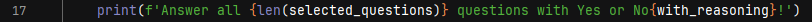
\includegraphics[width=1\linewidth]{graphics/Answer-all-questions-with-reasoning.png}
	      	\caption{A nagy nyelvi modellek promptját úgy kezdtem, hogy érveljen minden mondat esetében.}
	      	\label{fig:enter-label1}
	      \end{figure}
 Tapasztalatom szerint ez elég volt ahhoz, hogy részletes válaszokat kapjak a modellek webes futtatása esetében, de lokális futtatásnál is segített tájékozódni.
\end{enumerate}

\subsubsection{Egyszavas válaszok}
A szótárból előállított prompt formátuma pedig a következő:
\begin{verbatim}
Answer all `n` questions with Yes or No!
Does the word "defeat" mean the same thing in sentences
"It was a narrow defeat." and "The army's only defeat."?
Does the word "groom" mean the same thing in sentences
"Groom the dogs." and "Sheila groomed the horse."?
.
.
.
(n sor összesen)
\end{verbatim}

A modellek erre a formátumra szinte mindig csak egy $Yes$ vagy $No$ szóval válaszolnak, ezt saját teszteléssel is megerősítettem. Ezeket az előrejelzéseket egy egyszerű \texttt{Yes -> T, No -> F} leképezéssel össze lehet hasonlítani a gold fájlokban található igazat és hamisat jelölő $T$ és $F$ címkékkel.


Eltérő kimenetet kapok, ha érvelés kérésével adom be a modelleknek a szöveget:
\begin{verbatim}
Answer all `n` questions with Yes or No with reasoning!
Does the word "defeat" mean the same thing in sentences
"It was...
\end{verbatim}

Ebben az esetben a chatbotok 1-2 mondatban meg szokták magyarázni a döntésük mögötti logikai érvelést. Ez is hasznos információ, amelyet felhasználok a modell teljesítményének megítéléséhez.

\vspace*{1cm}
A modellek válaszát egy Google táblázatba mentettem el. Az első oszlopban jegyeztem fel a szavakat az adathalmazokból, a másodikban a gold standardot, a rákövetkezőkben pedig a modellek válaszait. Az adatok alatt összesítettem egy pár releváns adatot, többek között a pontosságot, kiegyensúlyozott pontosságot és az egyenesen és fordított sorrendben beadott mondatok egyezési arányát. Előbbiekhez beépített Google Táblázatok függvényeket használtam, míg utóbbihoz \href{https://script.google.com/home/}{Apps Scriptet}, a Táblázatok egy bővítményét, amellyel saját függvények definiálhatók és használhatók a táblázat bármely cellájában.
% \begin{figure}[H]
% 	\centering
% 	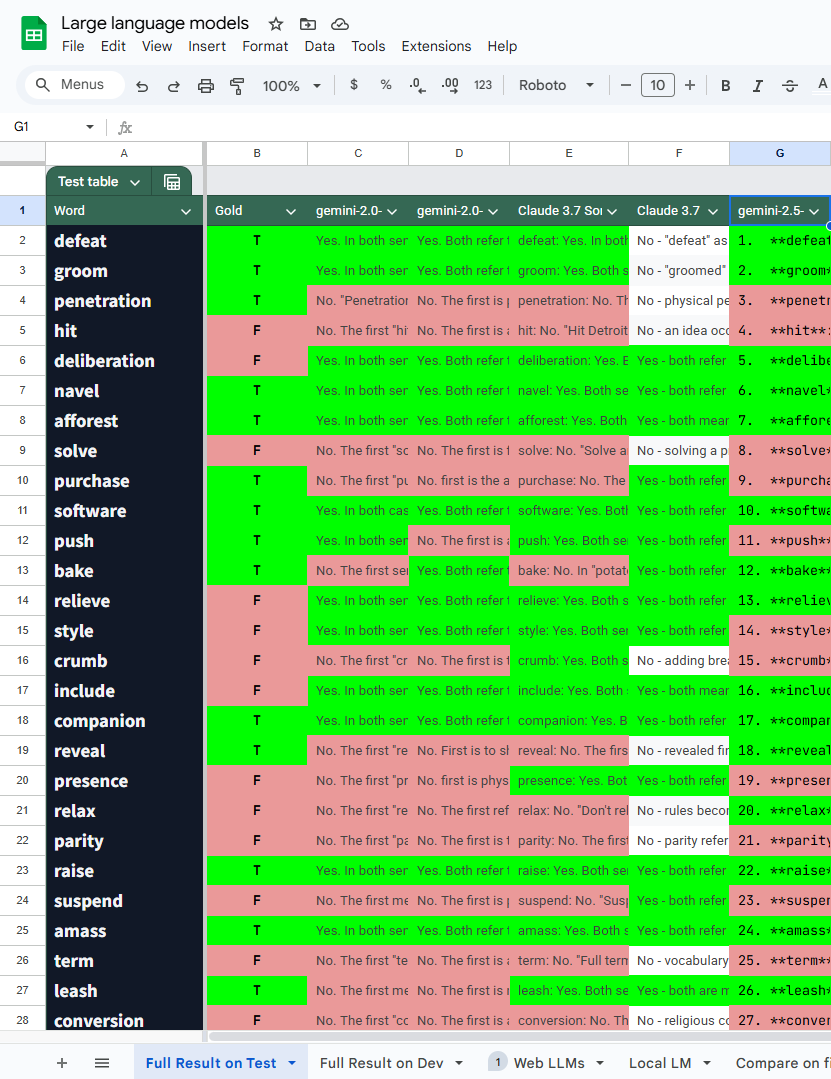
\includegraphics[width=1\linewidth]{graphics/sheets-large-language-models-main-page-demo-1.png}
% 	\caption{A tesztadatok és rajtuk végzett predikciók Google táblázatban}
% 	\label{fig:sheets-prediction}
% \end{figure}

% \begin{figure}[H]
% 	\centering
% 	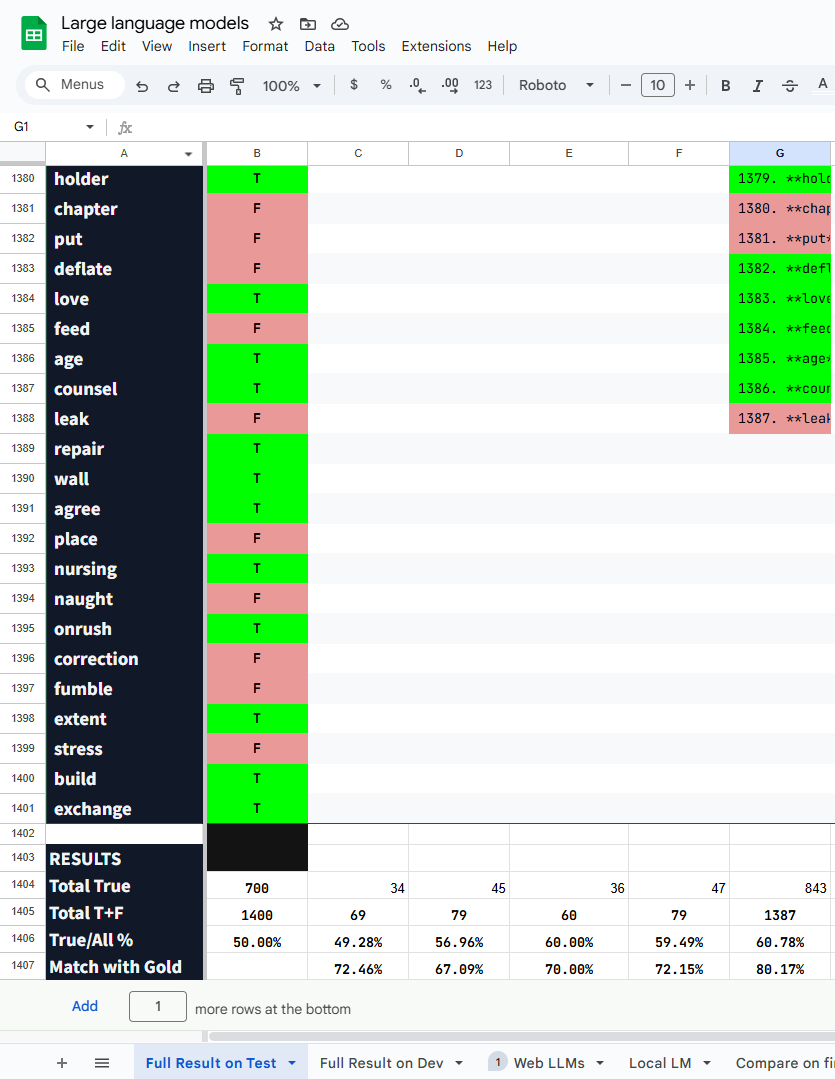
\includegraphics[width=1\linewidth]{graphics/sheets-large-language-models-main-page-demo-2.png}
% 	\caption{A predikciók összesítése és pontosság számolás Google táblázatban}
% 	\label{fig:sheets-prediction}
% \end{figure}


Az első sorban szerepelnek a gold standard értékek.
A TP, FP, FN, TN címkék számát és eloszlását a Google Táblázatok beépített függvényei segítségével határoztam meg, és szimplán összeszámoltam a modellek által predikált "Yes" és "No" válaszok soronkénti megegyezését az azonos sorban szereplő gold standard értékekkel.

Egyes modelleknél (pl. Gemini 2.5 Pro Experimental 03-25) problémát okozott az, hogy nem szerepelt a válaszában sem 'Yes', sem 'No', illetve előfordult az is, hogy nem csupán egy 'Yes', vagy egy 'No' válasszal tért vissza, hanem gondolatmenetet, magyarázatot is hozzáfűzött - akkor is, ha a promptban ennek az elhagyására kértem. % Így pl. az "I know! The answer is Yes." szöveg a Google Táblázatok függvényemben 'No'-ként lenne beleszámítva, akkor is, ha utána a modell szerint.
Emiatt ezeknek a modellek outputjának a feldolgozását manuálisan végeztem.
% \begin{figure}[H]
% 	\centering
% 	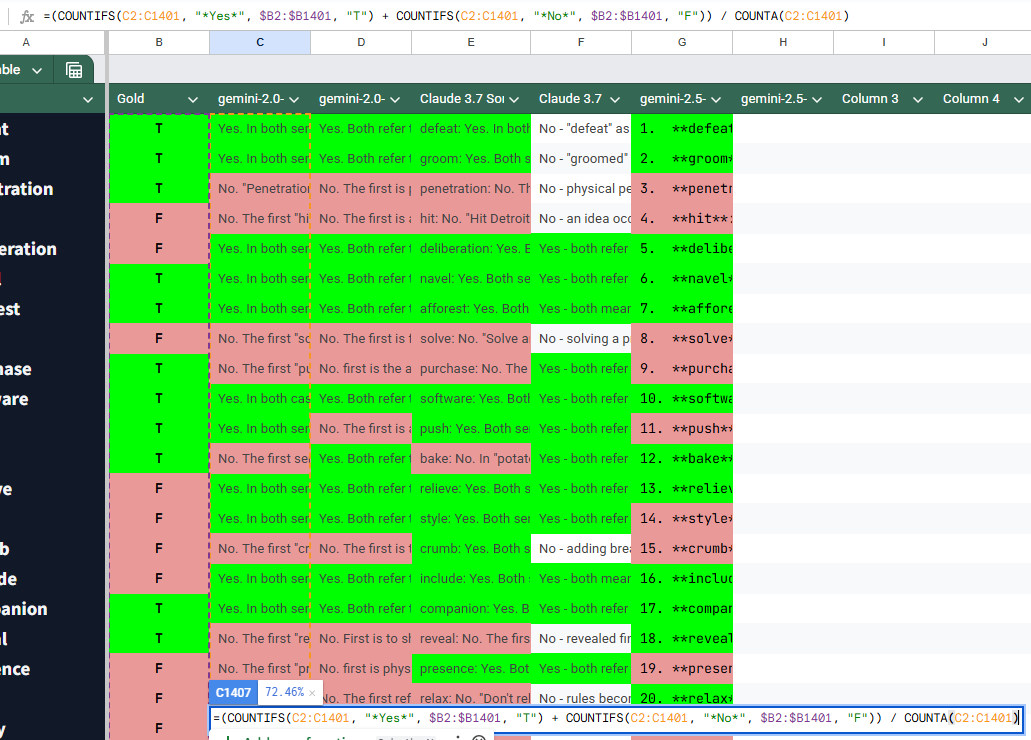
\includegraphics[width=1\linewidth]{graphics/sheets-regex.png}
% 	\caption{Reguláris kifejezések használata a válaszok kinyeréséhez}
% 	\label{fig:enter-label}
% \end{figure}

%\vspace*{2cm}

\subsubsection{A WiC saját kézi kiértékelése}
A \href{https://pilehvar.github.io/wic/}{WiC honlapján} az áll, hogy az emberi, manuális kiértékeléssel körülbelül 80\%-ot tudtak elérni, azaz 80\%-os pontossággal tudták a teszt adathalmazból vett, véletlenszerű példákról megállapítani, hogy a szó a 2 mondatban ugyanazt jelenti-e (a gold standard alapján). Ez nem túl magas, de érthető, tekintve, hogy ezek többsége ritka szó, és a mondatok nyelvezete is sokszor régies, vagy nagyon tudományos. A módszer az volt, hogy minden annotátor kapott 100 példát, és semmilyen segédeszközt nem használhattak.

Hogy meggyőződjek a nehézségről, én is eldöntöttem 60 bejegyzésről a gold standard ismerete nélkül, hogy a vizsgált szó ugyanazt jelenti-e a két mondatban. Az én eredményem 63.33\%-os pontosság és 63.17\%-os kiegyensúlyozott pontosság lett. Az eredményeim megtalálhatóak a kiértékelő rendszeremben a \texttt{manual\_evaluation} mappában.

% \subsubsection{ Megvizsgált modellek}
% A \href{https://lmarena.ai}{lmarena.ai} oldalon az 5 legnépszerűbb nagy nyelvi modellt teszteltem,  a \texttt{temperature}-t és a \texttt{top-p}-t 1-re állítva, a \texttt{maximum output tokens} paramétert pedig 4096-ra állítva. Ez maximális hosszúságú, determinisztikus válaszokat biztosított.

% A kontextusablakon kívül 2 nagyon fontos másik paramétert is lehet állítani.
% \begin{figure}[H]
% 	\centering
% 	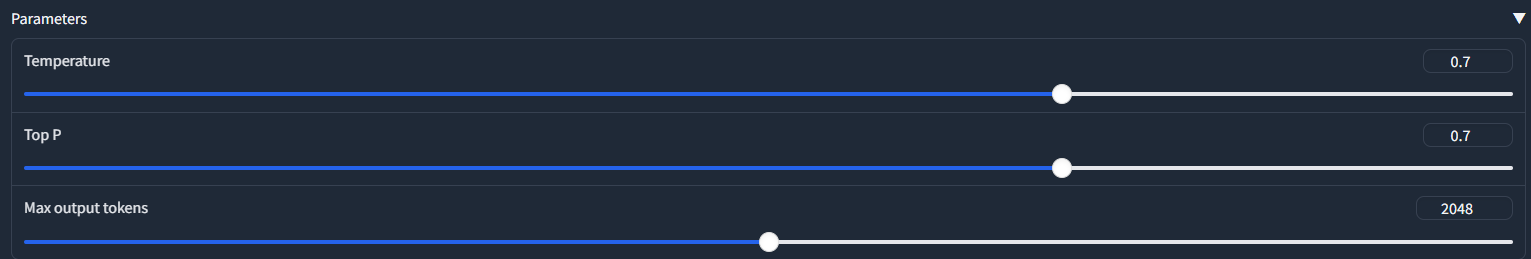
\includegraphics[width=1\linewidth]{graphics/lmsys-direct-chat-parameters.png}
% 	\caption{A nagy nyelvi modellek konfigurása a prompt beküldése előtt.
% Lmsys direct chat állítható paraméterei a top-p és a temperature segítségével kizáarható a véletlen válaaszadás}
% 	\label{fig:enter-label}
% \end{figure}
% Ez a nagymértékű személyre szabhatóság vonzóvá tette számomra a LMArenát.

% A \href{https://lmarena.ai}{lmarena.ai} webalkalmazáson kívül a nyelvi modelleket fejlesztő vállalatok hivatalos oldalain található modell legújabb verzióit is teszteltem, hogy mennyire jól oldják meg a WiC feladatot. Az alábbi táblázat tartalmazza a használt platformokat és a tesztelt modelleket, platformonként.
% A LMArenán kívül rengeteg nagy cég kínál ingyenes, vagy fizetős API-t a legjobb nyelvi modelljeihez, melyekhez általában ingyenes webes felület található, ahol általános célú generatív mesterséges intelligenciával lehet csevegni, akár képi, hang- vagy videóalapú formában is. Ezeknek a legfőbb előnye a lokális modell futtatással szemben, hogy kényelmesek, gyorsak, és alig veszik igénybe az eszközünk erőforrásait - megjegyzendő, hogy egy gyenge minőségű általános célú nagy nyelvi modell futtatásához is ipari mennyiségű hardverre és erőforrásra van szükség.

% Azonban sok hátrányuk is van. Sajnos azt kellett észrevennem, hogy ezek a személyes, vagy munkahelyi használatra tervezett platformok nem, vagy alig konfigurálhatóak. Emiatt alig javítható az általuk elért eredmény, és ha javul is, az inkább az emlékező képességüknek köszönhető. A modell másik felhasználó számára, illetve másik környezetben ugyanazokat a hibákat követi el, mint a személyes betanítás előtt. További probléma a nagy nyelvi modellek hivatalos platformjaival, hogy az algoritmus működésébe - vagy a mai modelleknél már úgy is mondhatjuk, hogy a nagy nyelvi modell \textit{gondolkodásába} - nincsen megfelelő mértékű betekintése a fejlesztőnek. Ezt a problémát igyekszenek kiküszöbölni pl. a Gemini-flash-thinking verziók, vagy a DeepSeek-R1 "részletes magyarázatot nyújtó" modelljei, azonban ez sem ad kellő irányítást.
% Másik hátrányuk ezeknek a cloud-alapú chat API-knak, hogy folyamatosan adatot gyűjtenek a felhasználótól, amelyet felhasználnak a modelljeik tanítására, és akár harmadik félnek is kiadhatják. Emiatt semmilyen bizalmas adatot nem érdemes megadni ezeken a felületeken.



\subsubsection{Futtatás Google Colab felületen}
Ahhoz, hogy nagy nyelvi modell válaszait emberi időben megkapjuk, anélkül, hogy órákig felhasználnánk a személyi gépünk teljes erőforrását, GPU-n kell futtatni a modellt. Ez töredékére csökkenti a futási időt. Az általam elérhető eszközök egyike sem GPU-s. Erre kínált megoldást a Google Colab. Ez a platform segítségével távoli, Google szerverek gépjeit használhatjuk,  nem kell a gépünk háttértárát, memóriáját stb. használni saját szkriptjeink futtatásához, és akár GPU-s futtatókörnyezetet is használhatunk, áthidalva a gépünk hardveres korlátait. Hátrányai, hogy a programunk változói, memóriája csak a session erejéig tárolódik, és lassabb futásidejű, mint a lokálisan futó program. A hátrányain úgy kerekedtem felül, hogy AutoClicker szoftvert állítottam a jegyzetfüzet egy véletlenszerű pontjára, így életben tartva az aktív munkamenetet akár órákig is.




\subsection{Eredmények}

Az összes pontosság és kiegyensúlyozott pontosság kiértékelésem 50\% és 62\% közötti eredményt ért el úgy, hogy mindegyik modell pontosan ugyanazt a promptot kapta. Leggyengébben a Phi szerepelt normál sorrendben (53.33\% és 56.03\%), fordított sorrendben (58.33\% és 60.71\%). A Gemma normál sorrendben (60.00\% és 61.83\%), fordított sorrendben (55.00\% és 56.47\%), eredményt ért el, míg a QWEN egyenes sorrendben (56.67\% és 57.37\%), fordított sorrendben pedig szinte azonos pontszámot ért el mindkét metrikában (58.33\% és 58.93\%). A kiegyensúlyozott pontosság magasabb, mint az egyezés mind a három modell esetében, ami azt sugallja, hogy egyenlő mértékben hajlamosak igennel és nemmel válaszolni. %A legjobb eredményt a "gemini-2.5-pro-exp-03-25 normal" (80.17\% 73.36\%) és a "gemini-2.5-pro-exp-03-25 reversed" (79.80\% 73.77\%) érték el. Ez a modell amellett, hogy rendkívül jól értette meg a szavak jelentését, a szavak sorrendjére sem érzékeny.

% Következtetéseket vontam le a gemma-2-2b-it és a Phi-4-mini-instruct válaszairól és a konzisztenciájukról, azaz hogy ha megfordítjuk a 2 mondat sorrendjét, akkor mennyire válaszolják ugyanazt, mint ha egyenes sorrendben adtam volna be. A gemma-2-2b-it nagyon rosszul teljesített a feladatra, kb. mindenre Yes-t mondott a 60 kérdésből, pár kivétellel, amelyekre viszont helyesen mondott No-t. Tehát a precizitása rendkívül magas, hiszen a True címkéket mind felismerte, azonban a fedése nagyon alacsony, mert amit igaznak gondolt, annak alig több mint a fele volt igaz. Ezzel szemben a Phi-nak körülbelül 55\% a precizitása, és a fedése is. A Phi-4-mini-instruct válaszai nagyjából helyénvalóak voltak.

A függelékben található táblázatban összesítettem a három nyelvi modell teljesítményét különböző nehézségű és sorrendű kérdések (normál és fordított) esetén, és konzisztenciájukat is feltüntettem. Az értékelés pontosság, kiegyensúlyozott pontosság és egyezés százalékban történt. A modellek viselkedése és erősségei/hátrányai a megjegyzések oszlopban is kiemelésre kerültek.[~\ref{tab:model-eval-summary}]

\subsection{A Phi erősségei}
A Phi-4-mini-instruct modell stabil és konzisztens teljesítményt nyújt, ahogy a megjegyzések is jelzik. A közepes nehézségű fordított kérdéseknél is viszonylag jó, 58.33\% pontosságot és 60.71\% kiegyensúlyozott pontosságot ért el.

\begin{table}[h]
    \centering
    \begin{tabular}{lcc}
        \hline
        & \textbf{Accuracy} & \textbf{Balanced Accuracy} \\
        \hline
        Közepes F & 58.33\% & 60.71\% \\
        \hline
    \end{tabular}
    \caption{A Phi Legjobb Eredményei}
    \label{tab:accuracy_balanced_accuracy1}
\end{table}

\subsection{A Phi gyengeségei}
Bár a Phi-4-mini-instruct stabilnak mondható, a közepes nehézségű kérdéseknél a pontossága viszonylag alacsony (53.33\% normál, 58.33\% fordított sorrendben), annak ellenére, hogy az egyezés rendkívül magas (94.92\%). Ez arra utal, hogy gyakran ugyanazt a hibát követi el, a szavak sorrendje nem befolyásolja őt különösebben a döntés meghozásában. Ez jó jel, hiszen azt jelenti, a modell képes a szavak sorrendjétől elrugaszkodni és absztraktabban, a feladat megoldására koncentrálva válaszolni. A nehéz kérdésekre pedig teljesen egyoldalúvá válik, és szinte minden idegen szó- és mondatkörnyezetet eltérő jelentésűnek kategorizál, tehát egyértelműen meghatározható ennek a modellnek a teljesítménykorlátja.

\subsection{A Gemma erősségei}
A gemma-2-2b-t modell a közepes és nehéz kérdések esetén is 10\%-kal felülmúlta a másik 2 modellt. Megfigyeltem egyébként, hogy a Gemma-2-2b-it helyes válaszai és hibái is nagyrészt megegyeznek a Gemma-2.5 válaszaival, ami bizonyítja az architekturális alapjuk hasonlóságát. A Gemma-2-2b-it a nehéz kérdésekre is 67\%-os arányban jól válaszolt, jóval felülmúlva ezzel a két másik megvizsgált modellt.
A Gemmának további előnye, hogy Colabos környezetben jóval gyorsabban fut, mint a Phi és a Qwen modellek, 1 perc alatt akár 60 kérdésre is képes válaszolni.

\begin{table}[h]
    \centering
    \begin{tabular}{lcc}
        \hline
        & \textbf{Accuracy} & \textbf{Balanced Accuracy} \\
        \hline
        Közepes N & 60.00\% & 61.83\% \\
        Nehéz N & 68.75\% & 72.22\% \\
        Nehéz F & 60.00\% & 55.56\% \\
        \hline
    \end{tabular}
    \caption{A Gemma Legjobb Eredményei}
    \label{tab:accuracy_balanced_accuracy2}
\end{table}


\subsection{A Gemma gyengeségei}
A gemma-2-2b-t modellnek nem találtam különösebb gyengeségét.

\subsection{A Qwen erősségei}
A Qwen1.5-1.8B-Chat a Gemmánál jobb teljesítményt nyújtott egyszerű kérdéseken.

\subsection{A Qwen gyengeségei}
A Qwen1.5-1.8B-Chat a nehéz kérdésekre a Qwen egyáltalán nem volt jó, és érdekes módon a Phi-vel ellentétesen, amely mindent a hamis kategóriába sorolt, a Qwen túlságosan megengedő és határozatlan volt, és a kérdések 84, majd 100\%-ában egyezőnek feltételezte a szavak jelentését a két mondatban.


\subsection{Összegzés}
Összességében elmondható, hogy a Gemma teljesített a legjobban a három modell közül. Pontos, nem preferálja aránytalanul az egyik osztályt, öntudatos, figyel a saját korábbi válaszaira és konzisztens is, azaz el tud rugaszkodni a szavak sorrendjétől, absztraktabb módon a feladaton tartja a fókuszt. Általános célú feladatokra, például egy programozási feladat megoldására sokkal rosszabbul teljesít, mint egy GPT-4o, Claude 3.7 Sonnet, Grok vagy DeepSeek modelljei. A gemma-2-2b-it nem általános célú modell, hanem elsősorban utasításkövetésre lett optimalizálva.


\newcommand{\chapterwithdesc}[2]{%
  \chapter{#1}%
  \vspace{-1ex}%
  {\large\itshape #2\par}%
  \vspace{2ex}%
}
\chapterwithdesc
  {A szoftver: Input előkészítő és output feldolgozó rendszer fejlesztése PyCharmban}
  {A részletes kimutatásokat tartalmazó megoldás}
\label{chap:src/Framework}

A szoftvert, amelyet a szakdolgozatomhoz készítettem, 2024-ben kezdtem el fejleszteni, és a mai napig fejlesztem GitHubon. A \href{https://github.com/Fabbernat}{GitHubomon elérhető a kitűzött elemek között}. Korábban a \href{https://github.com/Fabbernat/Peternity}{https://github.com/Fabbernat/Peternity} linken volt elérhető, ám ezt összezavarónak találtam, ezért áthelyeztem a \href{https://github.com/Fabbernat/Thesis} {https://github.com/Fabbernat/Thesis} linkre, és igyekszem onnan többet nem elmozdítani.

A projekt első verziója sokat lett kritizálva, hogy átláthatatlan és sok benne az AI generált, rossz minőségű kód, így 2025 nyarán újrakezdtem. Az új modulnak 2 fő fejlesztési szempontja volt.

Az egyik, hogy a teljes "WiC adathalmazból modell prompttá", továbbá a modell outputból adatkinyerés %TODO rephrase
folyamat egy helyen, egy kattintással elvégezhető legyen a Clean Code módszereivel.

A másik az, hogy a promptok alapjául szolgáló adathalmaz és a modellek nagyon egyszerűen cserélhetőek legyenek, anélkül, hogy a program egyéb részein módosítani kellene.


A projekt kutatási szempontból érdekes része így csak az újraírt \textit{src/Framework} modulban található. A többi archívum és mellékelhető a projekt megértéséhez. A \textit{src/Framework} 3 almodult tartalmaz, amelyek mindegyike egy önálló, de nagyon egyszerűen futtatható programot tesz ki. Egyesítve is lehet futtatni, de több indoka is van, hogy miért inkább egyesével érdemes futtatni a programokat. Az első és utolsó modul offline futtatható és nem erőforrásigényes, a hibák esélye minimális. A középső modul a fő ok, amelyben rengeteg a hibaforrás és a nemdeterminizmus. Online API hívásokat végez és GPU-t igényel (GPU hiányában pedig hatalmas erőforrásigényt és számítási kapacitást), ráadásul sok 3rd party library-ra támaszkodik. Emiatt érdemes külön futtatni ezt a programot és a hibákat lekezelni. a modulok futtatási sorrendje fontos.

A ModelInputPreparer, amely a WiC adathalmazból létrehozza a modellnek szánt inputot, az 5600 kérdést. Ez a 'WiC adathalmaz' 'test' splitjének összes rekordjából létrehoz egy kérdést, mind egyenes, mind fordított sorrendben, hogy a modellek konzisztenciáját vizsgáljuk. Mivel 2800 rekordból áll, és rekordonként 2 kérdésünk (egyenes, fordított) van, így jön ki az 5600 kérdés.

% TODO
A CloudRunnerNotebooks ...



A ModelOutputProcessor ...



\section{Technológiák}
\begin{itemize}
\item NLTK WordNet – szóértelmezéshez

\item SentenceTransformer – BERT-alapú mondatembeddinghez

\item TF-IDF, cosine\_similarity – szövegösszehasonlításhoz

\item scikit-learn – küszöboptimalizálás, értékelés
\end{itemize}

Még mielőtt belekezdenék a tervezési gondolatmenetem kifejtésébe, hadd említsem meg, hogy miért ezeket a technológiákat használtam.

\subsection{Az NLTK}
Az NLTK (Natural Language Toolkit)~\cite{bird2004nltk} egy Python könyvtár, amely számos természetes nyelvfeldolgozási eszközt és adatkészletet kínál. Az NLTK kínál egyszerű eszközöket szójelentés-egyértelműsítésre, mint amilyen a korábban említett Lesk algoritmus implementációja, melyhez a WordNet~\cite{miller1994wordnet} szolgáltatja a szükséges lexikális adatbázist.

A WordNet egy nagy lexikális adatbázis, amely angol nyelvű szavakat csoportosít úgynevezett "synset"-ekbe, amelyek kognitív szinonimákat és szavak közötti szemantikai kapcsolatokat is tartalmaznak. Minden synset egy fogalmi jelentést reprezentál, és a különböző synset-ek különböző jelentéseket fejeznek ki. %A Lesk algoritmus egy klasszikus WSD módszer, amely a vizsgált szó környezetében lévő szavak és a WordNet-ben szereplő definíciók közötti átfedés alapján határozza meg a legvalószínűbb jelentést.
A WordNet letöltését és elérhetőségének ellenőrzését a \texttt{download\_wordnet\_if\_needed} függvénnyel automatizáltam. A szinonimák és jelentések kinyerésére a \texttt{get\_synonyms} függvényt alkalmaztam, amely egy adott szóhoz tartozó összes lehetséges szinonimát visszaadja a WordNet segítségével. Az \texttt{expand\_with\_synonyms} függvény pedig egy teljes mondat szemantikai kiterjesztését végzi el, ami segítségével a mondatok közötti szemantikai átfedések explicit módon vizsgálhatóvá váltak.

\subsubsection{A WiC modell működése}
A modell egy előtanított nyelvi modellt használ, amely képes a szóhasználatok közötti finom eltéréseket azonosítani. A bemenet két mondatból és a vizsgált szóból áll, míg a kimenet egy bináris döntés: azonos vagy eltérő jelentés.

\subsubsection{Adatfeldolgozás és annotáció}
Az adatok előkészítése során szükség van megfelelő annotációs technikák alkalmazására. Az adatkészleteket standard WiC benchmarkokból nyerjük, amelyek kézi annotációval lettek ellenőrizve.

\subsection{BERT}
A BERT lényegében egy, a modellek reprezentációs képességét segítő szóbeágyazás, amely dinamikusan képes a mondatokhoz reprezentációt létrehozni. Ez nagy előny a régebbi, jól ismert statikus szóbeágyazásokkal szemben, mint például a Word2vec és a GloVe. Utóbbiak ugyanis egy szóhoz ugyanazt a szóvektort rendelik, bármilyen szövegkörnyezetben fordul is elő. A legnagyobb probléma ezzel, hogy sok szónak több, teljesen eltérő jelentése van, ám ezek a szóbeágyazások képtelenek modellezni szavak szemantikájának ezt a dinamikus természetét. A BERT ezzel szemben úgy hozza létre a mondatreprezentációt, hogy figyel a szövegkörnyezetre akár predikálás közben is. Ezzel lehetővé teszi, hogy ha egy szónak, vagy mondatnak több értelme is van, azt képes legyen a kontextus és a szó figyelembevételével megkülönböztetni.


A word2vec egy mára már elavultnak tekinthető technológia, ezért nem használtam, de a transzformerek megértéséhez hozzásegített.


Az utóbbi évek fejlődésével az olyan mélytanulási modellek, mint a BERT (Bidirectional Encoder Representations from Transformers) és más transzformátor-alapú nyelvi modellek még fejlettebb szövegreprezentációt kínálnak, figyelembe véve a kontextust és a szavak közötti összefüggéseket.






\section{Tervezés}

\subsection{A kiértékelő rendszer célja}
A készített alkalmazás célja az adatfeldolgozáson kívül, hogy egy olyan kiértékelő algoritmust hozzak létre, amely a Word-in-Context (WiC) feladatokhoz nyújt támogatást, lehetővé téve a szavak kontextusbeli jelentésének hatékony felismerését és osztályozását, továbbá minél nagyobb pontosságot ér el a \href{https://pilehvar.github.io/wic/package/WiC\_dataset.zip}{WiC - The Word in Context Dataset} teszthalmazon.
A Google Colab jegyzetfüzetemhez hasonlóan itt is Pythont választottam, mert hatalmas a könyvtártámogatása NLP és mesterséges intelligencia területen, ami különösen alkalmassá  teszi gyors fejlesztésre és adatfeldolgozásra, különösen szöveges adatokéra. Ezen kívül egy könnyen olvasható, általános célú, egyszerű szintaxisú, magas szintű programozási nyelv. Fejlesztői környezetnek a  PyCharmot használtam.

Célom volt, hogy a kiértékelő rendszerem
% ne használjon abszolút útvonalakat és lokális fájlokat, és hogy annak
almappái egy önálló modulként használhatóak és futtathatóak legyenek - a környezet megfelelő felállítása után.

Fő szempontjaim voltak, hogy a projekt fájlstruktúrája könnyen értelmezhető legyen, kövesse a konvenciókat, könnyen lehessen benne tájékozódni, és logikusan legyen felépítve. Emellett a Python szkriptek, amennyire csak lehet, ne függjenek egymástól, tehát önállóan futtathatók legyenek. Természetesen ettől indokolt esetben eltértem, például amikor nagyméretű adatokat tároltam egy fájlban, azt másik rövid szkriptekben használtam fel, a könnyebb átláthatóság kedvéért.

\subsubsection{Fájlstruktúra}
A projektemben megtalálhatóak a Python projektekhez elengedhetetlen .venv (Virtuális Python környezet), requirements.txt a dependency-k követéséhez, Git fájlok (.gitignore, README, .git), és a fejlesztői környezet fájljai (.idea). Ezek nem érdekesek most számunkra. Az azonosítók elnevezését is igyekeztem rendkívül konzisztensen végezni: minden külső használatra szánt, úgynevezett "utility"  Python szkriptem a \texttt{wic}  előtaggal kezdődött. Amelyik pedig belső használatra volt szánva, vagy szabványos neve van (pl. \_\_init\_\_.py, setup.py), az nem kapott \texttt{wic}  előtagot.
Az ötletet többek között az Intel által fejlesztett OpenCV \texttt{cv2} digitális képfeldolgozásra szolgáló függvénykönyvtárából merítettem, amely többek között Python nyelven is használható. Itt ugyanis minden beimportálható függvény, enum, változó, konstans stb. a \texttt{cv2}. előtaggal kezdődik, amely rendkívül megkönnyíti a \texttt{cv2} azonosítóinak (Függvény-, Osztály-, Változó-, Konstans-, Metódus-, Paraméter-, Enum- és Névtérnevek) elkülönítését a saját azonosítók, és ezáltal elősegíti a kód olvashatóságát.


\subsubsection{"Pythonic" alapelvek}
A projektemben igyekeztem követni a \href{https://peps.python.org/pep-0020/}{Zen of Pythonban}~\cite{peters2004zen} megfogalmazott, "Pythonic" alapelveket és a Python közösség által elfogadott jó gyakorlatokat.
A Pythonic elveket úgy alkalmaztam, hogy minél több információt expliciten adtam meg, funkcionálisan programoztam, kerülve a beágyazott blokkokat, és elősegítve a kód önmagát dokumentáló jellegét. A kódomban előforduló azonosítóknak, főleg a fájloknak, változóknak, függvényeknek rendszerint hosszú, \textit{barokkosnak} nevezhető nevet adtam, hogy a fájl megnyitása nélkül is világos legyen, hogy mit csinál, miért felelős. A rendkívül hosszú azonosítónevek adása egyébként a nagyvállalati kultúrában, a Java és a legtöbb, objektumorientált nyelvet használó programozók körében is bevált konvenció, hiszen többek között csökkenti a dokumentáció szükségességét. Az összetett logikát egyszerűbb, egymás után következő lépésekre bontottam le, még ha ez kódismétléssel is járt, a könnyebb olvashatóság érdekében.

\subsubsection{A projekt felépítése}
A tervezés során számos lépést megtettem, hogy a projektem könnyen átlátható legyen:
\begin{itemize}

	\item Mivel a szkriptjeim nagy részében több ezer soros fájlok adataival dolgoztam, és nem lett volna célszerű minden fájlba közvetlenül importálni ezt a nagy adatmennyiséget, ezen kívül környezettől függetlenül futtathatóvá akartam tenni a projektem, ezért automatizáltam az importálási folyamatot, és változókban mentettem el a fájlneveket és az elérési útvonalakat, amely szinte az összes (nem csak függvényeket tartalmazó) szkriptemben állítható az \texttt{actual\_working\_dataset} változóval.
	\begin{figure}[H]
		\centering
		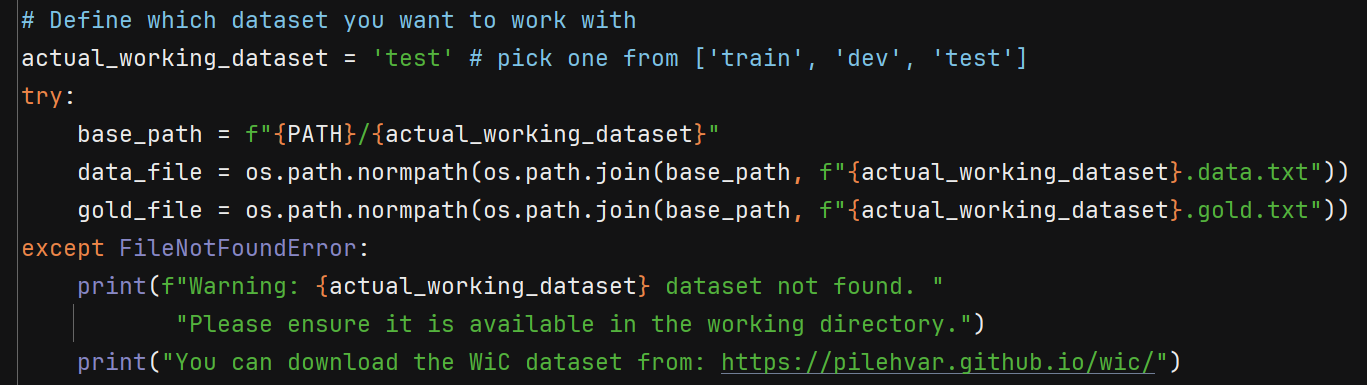
\includegraphics[width=1\linewidth]{graphics/automate-choosing-actual-working-dataset.png}
		\caption{Az adathalmaz kiválasztásának automatizálásának módszere}
		\label{fig:enter-label2}
	\end{figure}

	\item A harmadik féltől származó könyvtárak, csomagok és egyéb függőségek egységesen, \texttt{requirements.txt}-ben lettek definiálva. Ez egy Pythonos konvenció, amelyet én is követtem. A PyCharm eszközt kínál a projekt függőségeinek automatikus összegyűjtésére, és arra is, hogy a felhasználó egy gombnyomásra képes legyen ezeket egyszerre letölteni.

	\item \textbf{Modularitás:} A projektemben a lehető legkevesebb fájlokon átívelő függőséget alkalmaztam, tehát a projekt kódja annyira moduláris, amennyire csak lehet. Ez különösen hasznos a projekt kódjának refaktorálásakor, illetve akkor, ha csak egy, vagy pár fájlt kellett használnom a projektből egy bizonyos feladatra, mert biztosította a program kis méretét és gyorsaságát.
	\item
	      Kivétel erre a nem importálásra szánt fájljaim, ahol ténylegesen történik a függvények meghívása a saját függvénykönyvtár fájljaimból, és a konfigurációs beállítások (pl. Elérési utak) tárolására szolgáló fájljaim.
\end{itemize}

Figyeltem a SOLID objektum-orientált programozási alapelvekre~\cite{oloruntoba2024solid} is, főleg az Open-Closed alapelvre, hogy az alkalmazásom könnyen bővíthető, de nehezen elrontható legyen. A függvényeimet úgy paramétereztem, hogy úgy lehessen a kiértékelés módját változtatni, hogy csak 1 paramétert kell átírnunk hozzá, ezzel sok kódduplikálást megelőzve. Példák:
A \texttt{compute\_sentence\_similarity} alapértelmezett módon a gyengébb, nagyon gyors TF-IDF vektorizáló módban, azonban a \texttt{mode="bert"} paraméterezéssel a nagyon lassú, de sokkal jobb teljesítményű SenseBERT beállítással fut le, amely az említett előtanított nyelvi modellt használja, amelyet kifejezetten a szóérzékelés (word sense disambiguation, WSD) feladatra optimalizáltak.

Másik példám, ahogy az \texttt{evaluate} függvény alapértelmezetten a hibahatár threshold kísérletező paraméterével végigpróbálja az összes temperature-t, és automatikusan a legjobb eredményű kiértékelést választja. Ez hatékony, de nagyon sok időt vesz igénybe, ezért a paraméternek explicit értéket lehet adni. Ekkor csak erre az egy értékre fut le, ami gondos kiválasztást igényel a fejlesztő részéről, de nagyon gyors.
Még egy példa, hogy az eredmény-kiíró függvényben meg lehet adni bőbeszédű és normál opciókat, amellyel kiválaszthatjuk, hogy mennyi üzenet jelenjen meg a konzolon, és az elfogadható bizonytalanság mértékét is lehet állítani. Ugyanitt egyesével is tudjuk állítani a paraméterek kiíratását.

\subsubsection{Kommentek}
Angol nyelvű projekt lévén a kommenteket egységesen angolul írtam mindenhol, ez segítette az internetes segítségkérést, például fórumokon.

\vspace*{1cm}

\section{Implementáció}
Első lépésként inicializáltam a projektemet lokálisan és a GitHub verziókövető platformon. A program fejlesztését inkrementális modellel végeztem, tehát kezdetben csak vázlatosan határoztam meg a kiértékelő rendszer funkcióit. Ennek a modellnek az előnye például a vízesés modellel szemben az, hogy a követelmények nincsenek konkrétan lerögzítve a fejlesztés elején, hanem folyamatosan lehet rajtuk változtatni. Ha eszembe jut egy újabb módszer, amivel jobb eredményt lehet elérni, vagy egy funkció, amely növeli a program érthetőségét, átláthatóságát, akkor nem kell újratervezni a programot.
% \begin{itemize}
% 	\item BERT beágyazások
% 	\item Python algoritmusok, melyek Yes/No döntéseket hoznak
% 	\item Python algoritmusok, melyek előállítják a promptokat, amelyek inputként adhatók döntéshozásra nyelvi modelleknek
% \end{itemize}

\subsection*{ Mappák}
\begin{itemize}
	\item \textbf{independent\_scripts mappa}\\
            Az önállóan működő, független Python szkripteket ide raktam.
	\item \textbf{llm\_prompts mappa}\\
	      Az llm\_prompts mappában lévő szkriptekkel olyan promptokat hoztam létre, amelyektől jó eredményt lehet elvárni a nyelvi modelleken való promptolás esetén. Emiatt nyelvtanilag helyesek, a tokenek egymástól egyértelműen elkülönülnek, és szerkezetileg megfelelnek a nyelvi modellek elvárásainak: a prompt elején van az utasítás, majd a kérdések következnek jól elkülönülve.
	      A validáció és tesztelés érdekében készítettem pár nagyon egyszerű, és pár nagyon nehéz kérdést is a nagyon gyenge, illetve nagyon jól teljesítő modellek számára.

	\item
	      \textbf{modules\_and\_data mappa}\\
	      Ez a mappa a projekt futtatásához szükséges modulokat és az adathalmazokat tartalmazza.
	      2 részre oszlik:

	      \texttt{modules}: Ide tartoznak az adathalmaz tisztítását, felesleges, vagy használhatatlan adatok kiszűrését és egyéb adattranszformációkat végző Python szkriptjeim.

	      \texttt{data}: Az adatok előfeldolgozása és átalakítása ebben a mappában történik, például tokenizálás, normalizálás vagy TF-IDF számítás.

	\item
	      \textbf{solution mappa}\\
	      Szintén 2 részre oszlik\\
	      \texttt{Implementation}: Ez a mappa tartalmazza a megoldásom végső implementációját és a projekt által generált eredményeket. Itt található a BERT-alapú megoldásom, valamint a generatív nyelvi modellek teljesítményének összehasonlítása.

	      \texttt{Results}: Az itt található fájlok a különböző modellek által generált válaszokat, tévesztési mátrixokat, statisztikákat és egyéb mérőszámokat tartalmazzák.

          Ez az önálló, fájlokra szétbontott, TF-IDF-alapú megoldás a \texttt{main.py} szkripttel indítható. Ez a kiértékelő szkript a pontosság mellett kiszámítja és megjeleníti a precizitást, fedést és F1 pontszámot, valamint vizuálisan ábrázolja a tévesztési mátrixot.

	\item
	      \textbf{use\_modell\_locally mappa}\\
	     A \texttt{py} almappában webes API-on keresztül tesztelhetők az OpenAI és az Anthropic modelljei. A kód a fejlesztő cégek hivatalos modell dokumentációjából erednek. Az első szkripttel GPT modellek hívhatóak meg az OpenAI API-n keresztül az \href{https://platform.openai.com/docs/overview}{OpenAI dokumentáció}~\cite{openai2025api} által ajánlott módon egy adott szó jelentésének két mondatbeli összehasonlítására, míg a második fájlban ugyanilyen módon a Claude modelljei használhatók az Anthropic API segítségével az Anthropic dokumentáció szerint~\cite{anthropic2025api}.

	\item
	      \textbf{WiC\_dataset mappa}\\
	      A WiC (Word-in-Context) adathalmaz itt található

     \item     \textbf{demo\_files} mappa\\
A \textbf{demo\_files} mappában található egy alternatív kompaktabb megoldás, amely csak a pontosságot mutatja ki, de cserébe sokkal konfigurálhatóbb. \\A \texttt{wic\_tfidf\_or\_sensebert\_baseline\_single.py}\\
szkript egy alap Word-in-Context (WiC) probléma megoldására szolgáló baseline rendszert valósít meg, amely szóértelem-felismerésre (Word Sense Disambiguation, WSD) és mondat-hasonlóság számítására épít. Ez egy konfigurálható fájl, futtatásával a kiválasztott adathalmaz (train, dev vagy test) beolvasásra kerül, TF-IDF vagy SenseBert módban, opcionális kiírás-részletesség, küszöbérték- és szinonimaoptimalizálás beállításokkal.  A WordNet segítségével meghatározza a cél szó legrelevánsabb jelentését az adott mondat alapján, és csak a kontextushoz illő szinonimákat adja hozzá a mondathoz. TF-IDF és/vagy BERT-alapú mondatembeddingből egy hibrid hasonlósági értéket számol. Ezután meghatározza az optimális határértéket a "T"/"F" címkék elválasztásához, végül összehasonlítja a predikciókat a gold standard címkékkel, opcionálisan figyelembe véve egy bizonytalansági zónát. A legjobb eredményt a SenseBERT beállítással, legjobb threshold mellett, 19 perc futással értem el, mind a 3 halmazon 60\%-nál jobb eredményt értem el.
\end{itemize}

% \begin{table}[h]
%   \centering
%   \begin{tabular}{|c|c|c|}
%     \hline
%     Header 1 & Header 2 & Header 3 \\ \hline
%     Item 1   & Item 2   & Item 3   \\ \hline
%     Item 4   & Item 5   & Item 6   \\ \hline
%     Item 7   & Item 8   & Item 9   \\ \hline
%   \end{tabular}
%   \caption{Example Table}
%   \label{tab:example}
% \end{table}

\begin{table}[h]
    \centering
    \begin{tabular}{c|c|c|c}
    \hline
    Adathalmaz & Mód & Pontosság (\%) & Futásidő (másodperc) \\ \hline
        train & BERT & 59.912 & 8294.84 \\ \hline
        train & TF-IDF & 57.970 & 5903.44 \\ \hline
        dev & BERT & 60.696 & 128.44 \\ \hline
        dev & TF-IDF & 62.088 & 91.95 \\ \hline
        test & BERT & 59.571 & 382.36 \\ \hline
        test & TF-IDF & 60.658 & 332.65 \\ \hline
    \end{tabular}
    \caption{A \texttt{wic\_tfidf\_or\_sensebert\_baseline\_single.py} eredményei és futásideje a különböző beállítások mellett. Érdekes módon az egyszerűbb kérdéseket tartalmazó \texttt{train} halmazon a BERT jobban teljesít, míg a nehezebb kérdésekből álló \texttt{dev} és \texttt{test} esetén a TF-IDF minimálisan pontosabb. Ez alapján leszűrhető, hogy a BERT módszer egyszerűbb kérdések esetén hasznosabb, főleg ha nem lényeges a gyors a futásidő.}
    \label{tab:my_label}
\end{table}

\section{Tesztelés és eredmény}

\subsection{Kiértékelés}

\subsubsection{Klasszifikációs módszer}
Az algoritmusaim teljesítményét egy tévesztési mátrix segítségével, klasszifikációs módszerrel értékeltem ki, ami például Covid-teszt eredményekkel jól szemléltethető. Covid esetén pozitív a teszt, ha a páciens beteg, negatív, ha egészséges. Továbbá igaz a predikció, ha helyesen ítéltük meg az egészségi állapotát, és hamis, ha helytelenül ítéltük meg. Ezeknek a kombinálásával kapjuk meg a TP, FP, TN, FN értékeket.

\begin{figure}[H]
	\centering
	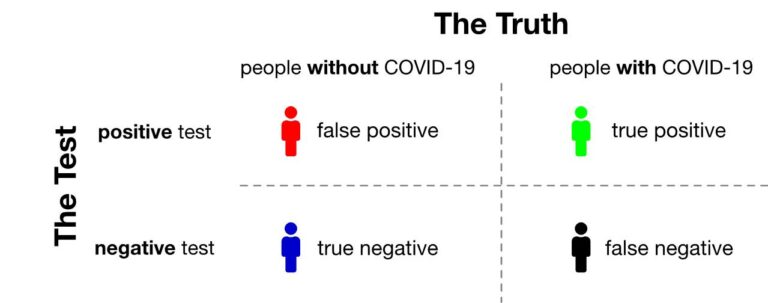
\includegraphics[width=1\linewidth]{graphics/covid-tp-tn-fp-fn.png}
	\caption{Covid-19 példa a TP, TN, FP, FN alkalmazására}~\cite{manrai2020covid}
	\label{fig:enter-label3}
\end{figure}

A WiC feladat esetében ezt úgy kell értelmeznünk, hogy pozitív a gold standard, ha a szó ugyanazt jelenti mind a két mondatban, negatív, ha eltérő dolgot jelent. Igazra értékelődik ki, ha helyesen ítélte meg a modell a szó jelentését és hamis, ha helytelenül ítélte meg. A modell válaszának a gold standarddal való összevetésekor minden esetet az alábbi négy kategória egyikébe sorolhatjuk:
\begin{itemize}
	\item \textbf{True Positive (TP):} A modell helyesen válaszol $Yes$-t, amikor a gold címke $T$, azaz valóban azonos a szó jelentése.
	\item \textbf{False Positive (FP):} A modell tévesen válaszol $Yes$-t, miközben a gold címke $F$, tehát eltér a szó jelentése.
	\item \textbf{False Negative (FN):} A modell tévesen válaszol $No$-t, miközben a gold címke $T$, tehát azonos lenne a szó jelentése.
	\item \textbf{True Negative (TN):} A modell helyesen válaszol $No$-t, amikor a gold címke $F$, azaz valóban különböző a szó jelentése.
\end{itemize}

\begin{equation}
	\begin{bmatrix}
		\text{Igaz pozitív (TP)}  & \text{Hamis pozitív (FP)} \\
		\text{Hamis negatív (FN)} & \text{Igaz negatív (TN)}
	\end{bmatrix}
\end{equation}


Az egyfájlos módszerem eredményei a 4.3. ábrán láthatók.~\ref{plot:traindevtest}
A kiértékelő rendszerem elérte a célját, hogy gyorsan ki tud értékelni több ezer kérdést, és legalább 60\%-os pontossággal el tudja dönteni a szavakról, hogy ugyanazt jelentik-e a 2 mondatban, vagy sem.

\subsubsection{Tanulságok, hipotézisek}
A WiC feladaton a természetes nyelvek szavainak szemantikájának komplexitásából adódóan gyakorlatilag lehetetlen 100\%-os pontosságot elérni, de ez nem is cél. Kézi, emberi kiértékeléssel 80\%-os eredményt lehetett elérni, a legjobb rendszerek pedig 70-72\%-ot értek el. A cél, hogy egy olyan WiC adathalmaz-kiértékelő szoftver készüljön, amely hosszú távon segít az embereknek, könnyen integrálható más projektekbe és széles skálán terjeszthető.

A kvantált modellek, mint a Gemma-2-2b-it, kisebb méretük miatt könnyebben futtathatók korlátozott hardveres erőforrásokkal, de ez a méretcsökkenés a teljesítmény rovására megy (pl. lassabb válaszidő, pontatlanabb eredmények).

A Gemma modell bizonyos specifikus feladatokra (pl. Word-in-Context) megfelelően alkalmazható, de általános célú kérdések esetén jelentősen alulmúlhatja a nagyobb modelleket, mint pl. GPT-4o vagy Claude.

A kis modellek érzékenyebbek a bemeneti prompt formátumára, mint a nagyok, különösen a sorrendiséget tekintve. Ha egy modellt ugyanarra a kérdésre eltérő sorrendű mondatokkal kérdezünk meg, akkor a válaszokban jelentős eltérések lehetnek. Emiatt az egyenként feltett kérdések pontosabb eredményt adnak, mint a több kérdést egyben tartalmazó prompt.

A nyílt forráskódú és offline futtatható modellek előnye, hogy teljes adatvédelmi kontrollt biztosítanak, mivel nem kommunikálnak a külvilággal, így érzékeny adatok feldolgozására biztonságosabbak.





% \chapter{A két módszer eredményei és ábrák}
% \section{Modell teljesítmény értékelésének módszere}

% A modell teljesítményét a pontosság , precizitás , fedés , F1 pontszám  mutatókkal értékeltem. ~\cite{SOKOLOVA2009427} A kapott eredményeket a \texttt{Matplotlib} és \texttt{Seaborn} grafikai Python könyvtárak segítségével ábrázoltam, a TP, FP, FN, TN értékek eloszlását pedig egy tévesztési mátrixszal .

% \vspace{1em}
% A \textbf{Pontosság} megadja az összes helyesen osztályozott eset arányát az összes vizsgált példához képest:



% A \textbf{Precizitás:} megadja, hogy a pozitívnak jelzett esetek közül hány volt valóban pozitív:

% \begin{equation}
% 	\text{Precizitás} = \frac{TP}{TP + FP}
% \end{equation}

% A \textbf{Fedés:} megadja, hogy a ténylegesen pozitív esetek közül hányat ismert fel helyesen a modell:


% \begin{equation}
% 	\text{Fedés} = \frac{TP}{TP + FN}
% \end{equation}


% \textbf{F1 pontszám:} a precizitás és a fedés alapján számítható harmonikus átlaga.
% \begin{equation}
% 	F_1 = 2 \cdot \frac{\text{Precizitás} \cdot \text{Fedés}}{\text{Precizitás} + \text{Fedés}} = \frac{2 \cdot TP}{2 \cdot TP + FP + FN}
% \end{equation}
% Ez a metrika kiegyensúlyozatlan osztályeloszlás esetén hasznos, amikor a pozitív és negatív címkék száma jelentősen eltér. Ilyen helyzetekben a sima pontosság félrevezető lehet, mivel egy primitív osztályozó magas pontosságot el tud érni úgy, hogy a gyakori osztályt minden esetben előre jelzi. Mivel a WiC-ben fele-fele arányban vannak a $True$ és $False$ címkék, ezért nincs nagy jelentősége.


%     \vspace*{2cm}

% \subsection{A részletes kimutatásokat tartalmazó, algoritmikus megoldás}
% \begin{center}
% 	{\Large\bf{Pontosság, Precizitás, Fedés, F1 pontszám és összesített statisztikák}}
% \end{center}



\subsection{Tanulságok, hipotézisek}
A WiC feladaton a természetes nyelvek szavainak szemantikájának komplexitásából adódóan gyakorlatilag lehetetlen 100\%-os pontosságot elérni, de ez nem is cél. Kézi kiértékeléssel 80\%-os eredményt lehetett elérni, a legjobb rendszerek pedig 70-72\%-ot értek el. A cél egy olyan WiC adathalmaz-kiértékelő szoftver, mely a jövőben felhasználható hasonló NLP- vagy adatfeldolgozási feladatokra, könnyen integrálható más projektekbe és széles skálán terjeszthető. Emellett persze a személyes célom volt a Python ismereteim fejlesztése is.

A Gemma modell bizonyos specifikus feladatokra (pl. Word-in-Context) megfelelően alkalmazható, de általános célú kérdések esetén jelentősen alulmúlja a nagyobb modelleket, mint pl. GPT-4o vagy Claude.

A kis modellek érzékenyebbek a bemeneti prompt formátumára, mint a nagyok, különösen a sorrendiséget tekintve. Ha egy modellt ugyanarra a kérdésre eltérő sorrendű mondatokkal kérdezünk meg, akkor a válaszokban jelentős eltérések lehetnek. Emiatt az egyenként feltett kérdések pontosabb eredményt adnak, mint a több kérdést egyben tartalmazó prompt.

A nyílt forráskódú és offline futtatható modellek előnye, hogy teljes adatvédelmi kontrollt biztosítanak, mivel nem kommunikálnak a külvilággal, így érzékeny adatok feldolgozására biztonságosabbak.

\subsection{Tervek a jövőre nézve}
Jövőbeli tervem ez a projekt után, hogy a XL-WiC~\cite{raganato2020xlwic} és a WiC-TSV~\cite{breit2021wictsv} problémát is mélyebben megismerjem, és lehetőleg magyar nyelvre is hasonló adathalmazokat találjak, és hasonló rendszert hozzak létre. Ezen kívül érdekes kísérlet lenne az, hogy a különböző méretű és tulajdonságú modellek többkörös beszélgetésben (multi-turn conversation) mennyire képesek következetesek maradni és önmaguknak nem ellentmondani.


\section{Összegzés}
Úgy gondolom, a szoftverem segíthet mindazoknak, akik hozzám hasonlóan nagy nyelvi modelleket szeretnének futtatni lokálisan egy Python környezetben, valamint akiket hozzám hasonlóan érdekel a nagy nyelvi modellek szemantikus képességeinek konzisztenciájának vizsgálata, és ehhez szeretnének megfelelő keretrendszert találni.
 Fontosnak tartom megjegyezni, hogy ez egy rendkívül gyorsan fejlődő iparág, így amit a szakdolgozatban állítok, az a jövőbeli olvasónak elévülhet.
A dolgozatomat úgy állítottam össze, hogy nyomon követhető és reprodukálható legyen, ezért nyílt forráskódú eszközökre (Python, GitHub, Hugging Face) és nyilvános adathalmazra (WiC) támaszkodtam.

\clearpage

\chapter*{Eredmények, ábrák}

\addcontentsline{toc}{section}{Eredmények, ábrák}
\begin{table}[H]
\centering
\label{tab:model-eval-summary}
\resizebox{\textwidth}{!}{
\begin{tabular}{|c|c|c|c|c|c|}
\hline
\textbf{Modell} & \textbf{Nehézség} & \textbf{Pontosság (\%)} & \textbf{Kiegy. Pontosság (\%)} & \textbf{Egyezés (\%)} & \textbf{Megjegyzés} \\
\hline
\multirow{6}{*}{Phi}
    & Közepes N & 53.33 & 56.03 & \multirow{2}{*}{95.00} &Legjobb egyezés, de alacsony pontosság \\
    & Közepes F & 58.33 & 60.71 & & \\
    \cline{2-3}\cline{5-6}
    & Nehéz N   & 53.33 & 44.44 & \multirow{2}{*}{60.00} &  \\
    & Nehéz F   & 60.00 & 52.78 & & Válasza szinte minden kérdésre "nem" \\
\hline
\multirow{6}{*}{Gemma}
    & Közepes N & 60.00 & 61.83 & \multirow{2}{*}{85.00} & Legpontosabb közepesekre \\
    & Közepes F & 55.00 & 56.47 & & \\
    \cline{2-3}\cline{5-6}
    & Nehéz N   & 68.75 & 72.22 & \multirow{2}{*}{73.33} & \\
    & Nehéz F   & 60.00 & 55.56 & & Legjobb nehéz kérdéseken is \\
\hline
\multirow{6}{*}{Qwen}
    & Közepes N & 56.67 & 57.37 & \multirow{2}{*}{91.67} & Erős egyezés \\
    & Közepes F & 58.33 & 58.93 & &  \\
    \cline{2-3}\cline{5-6}
    & Nehéz N   & 46.67 & 52.78 & \multirow{2}{*}{80.00} & \\
    & Nehéz F   & 40.00 & 50.00 & & Válasza szinte minden kérdésre "igen" \\
\hline
\end{tabular}
}
\caption{A három nyelvi modell teljesítménye különböző kérdésnehézségek és sorrendek mentén. N=normál, F=fordított (pontosság, kiegyensúlyozott pontosság és egyezés \%)}
\end{table}


\label{plot:traindevtest}
\begin{figure}[H]
	\centering
	\begin{verbatim}
        # Train dataset
        Evaluation Metrics:
        Accuracy: 52.819%
        Precision: 71.795%
        Recall: 9.285%
        F1 Score: 16.444%
        Correct predictions: 2867/5428
	\end{verbatim}
	\begin{verbatim}
        # Dev dataset
        Evaluation Metrics:
        Accuracy: 55.172%
        Precision: 61.074%
        Recall: 28.527%
        F1 Score: 38.889%
        Correct predictions: 352/638
    \end{verbatim}
    \begin{verbatim}
        # Test dataset
        Evaluation Metrics:
        Accuracy: 52.714%
        Precision: 57.540%
        Recall: 20.714%
        F1 Score: 30.462%
        Correct predictions: 738/1400
    \end{verbatim}
	\caption{A \texttt{solution} eredményei a train, dev és test halmazra}
	\label{fig:enter-label4}
\end{figure}


\begin{figure}[H]
    \centering
    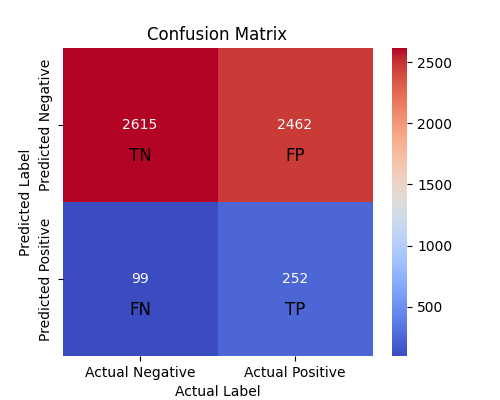
\includegraphics[width=0.5\linewidth]{graphics/WiC_confusion_matrix_abra.train.png}
    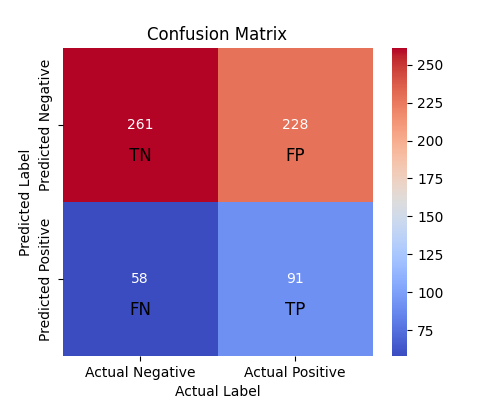
\includegraphics[width=0.5\linewidth]{graphics/WiC_confusion_matrix_abra.dev.png}
    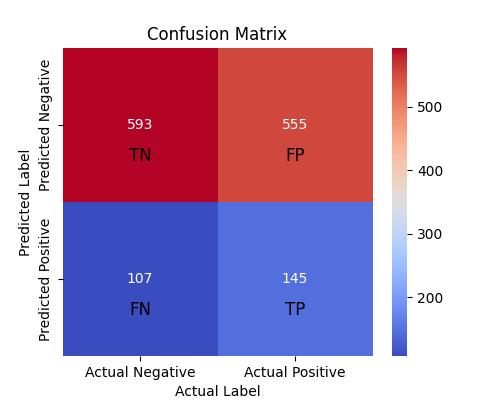
\includegraphics[width=0.5\linewidth]{graphics/WiC_confusion_matrix_abra.test.png}
        \caption{Az egyfájlos megoldás tévesztési mátrixai a train, dev és test halmazra}
    \label{fig:enter-label5}
\end{figure}


\clearpage

\label{fig:sentence-normalizer}
{\Large\bf Példa a sentence\_normalizer használatára}
\begin{lstlisting}
    # sentence_normalizer.py
    test_sentence = (
     r"My boss is out on another of his three martini lunches ."
     r" Will you join us at six o'clock for martinis ? We 've been swimming for hours just to get to the other side ."
     r" A big fish was swimming in the tank . Do n't fire until you see the whites of their eyes . The gun fired ."
     )

    print("Using NEW algorithm (default):")
    print(make_sentence_human_readable(test_sentence))
    # Output:
    # My boss is out on another of his three martini lunches. Will you join us at six o\'clock for martinis?
    # We\'ve been swimming for hours just to get to the other side. A big fish was swimming in the tank.
    # Don\'t fire until you see the whites of their eyes. The gun fired.
\end{lstlisting}


\medskip

\printbibliography

\chapter*{Nyilatkozat}
%Egy üres sort adunk a tartalomjegyzékhez:
\addtocontents{toc}{\ }
\addcontentsline{toc}{section}{Nyilatkozat}
%\hspace{\parindent}

% A nyilatkozat szövege más titkos és nem titkos dolgozatok esetében.
% Csak az egyik tipusú myilatokzatnak kell a dolgozatban szerepelni
% A ponok helyére az adatok értelemszerûen behelyettesídendõk es
% a szakdolgozat /diplomamunka szo megfeleloen kivalasztando.


%A nyilatkozat szövege TITKOSNAK NEM MINÕSÍTETT dolgozatban a következõ:
%A pontokkal jelölt szövegrészek értelemszerûen a szövegszerkesztõben és
%nem kézzel helyettesítendõk:

\noindent
Alulírott Fábián Bernát, programtervező informatikus BSc szakos hallgató, kijelentem, hogy a dolgozatomat a Szegedi Tudományegyetem Informatikai Intézet Számítógépes Algoritmusok és Mesterséges Intelligencia Tanszékén készítettem, a programtervező informatikus BSc diploma megszerzése érdekében.

Kijelentem, hogy a dolgozatot más szakon korábban nem védtem meg, saját munkám eredménye, és csak a hivatkozott forrásokat (szakirodalom, eszközök, stb.) használtam fel.

Tudomásul veszem, hogy szakdolgozatomat / diplomamunkámat a Szegedi Tudományegyetem Informatikai Intézet könyvtárában, a helyben olvasható könyvek között helyezik el.

\vspace*{2cm}

\begin{tabular}{lc}
	Szeged, \today\
	\hspace{2cm} & \makebox[6cm]{\dotfill} \\
	             & aláírás              \\
\end{tabular}


\vspace*{4cm}

%A nyilatkozat szövege TITKOSNAK MINÕSÍTETT dolgozatban a következõ:

% \noindent
% Alulírott \makebox[4cm]{\dotfill} szakos hallgató, kijelentem, hogy a dolgozatomat a Szegedi Tudományegyetem, Informatikai Intézet \makebox[4cm]{\dotfill} Tanszékén készítettem, \makebox[4cm]{\dotfill} diploma megszerzése érdekében.

% Kijelentem, hogy a dolgozatot más szakon korábban nem védtem meg, saját munkám eredménye, és csak a hivatkozott forrásokat (szakirodalom, eszközök, stb.) használtam fel.

% Tudomásul veszem, hogy szakdolgozatomat / diplomamunkámat a TVSZ 4. sz. mellékletében leírtak szerint kezelik.

% \vspace*{2cm}

% \begin{tabular}{lc}
% Szeged, \today\
% \hspace{2cm} & \makebox[6cm]{\dotfill} \\
% & aláírás \\
% \end{tabular}





\chapter*{Köszönetnyilvánítás}
\addcontentsline{toc}{section}{Köszönetnyilvánítás}

Ezúton szeretnék köszönetet mondani a családomnak, barátaimnak, tanítóimnak, tanáraimnak és egyetemi tanáraimnak, akik végigkísértek utamon és támogattak tanulmányaim alatt. Köszönetet szeretnék továbbá nyilvánítani szüleimnek, testvéreimnek és barátaimnak, hogy mindenben támogattak.

Végül, de nem utolsó sorban köszönetet szeretnék mondani \textbf{témavezetőmnek, Berend Gábornak}, hogy konzulensként és témavezetőként segített a szakdolgozatom megírásában.


%% Az irodalomjegyzek keszitheto a BibTeX segedprogrammal:
% \bibliography{diploma}
%\bibliographystyle{plain}


%VAGY "kézzel" a következõ módon:

% \begin{thebibliography}{9}
%10-nél kevesebb hivatkozás esetén

% \begin{thebibliography}{99}
% 	% 10-nél több hivatkozás esetén

	% \addcontentsline{toc}{section}{Irodalomjegyzék}

% 	%Elso szerzok vezetekneve alapjan ábécérendben rendezve.


% 	%folyóirat cikk: szerzok(k), a folyóirat neve kiemelve,
% 	%az evfolyam felkoveren, zarojelben az evszam, vegul az oldalszamok es pont.
% 	%könyv (szerzo(k), a könyv neve kiemelve, utana a kiado, a kiado szekhelye, az evszam es pont.)
% 	Az alkalmazás fejlesztése és elemzése során az alábbi forrásokra támaszkodtam:

    % Ez áthelyezné egy külső fájlba a referenciákat
	% \bibliographystyle{plain}
	% \printbibliography

% AUTHORS should prepare a .bib file for references but do not change the style file

\chapter*{Elektronikus mellékletek}
\addcontentsline{toc}{section}{Nyilatkozat}

\begin{itemize}
    \item
\label{att:colab}
A modelleket futtató Google Colab jegyzetfüzetem:
\href{https://colab.research.google.com/drive/1yA8IAd5z2oreKUXha-16Du2YrNhemNiU?usp=sharing}{ezen a linken}  található.
\item A program GitHubról a\\ \href{https://github.com/Fabbernat/Thesis}{https://github.com/Fabbernat/Thesis}\\ repozitóriumból tölthető le.
\item A nyelvi modellek tesztelése és kiértékelése a
\href{https://docs.google.com/spreadsheets/d/1y49lg52LHVFmTom-0ibCqYqWA1pKKhiUny-Pf3KVTIg/edit?usp=sharing}{Generative Language Models}
táblázatban tekinthető meg.
\end{itemize}


\end{document}